% ICLR 2027 submission. Started 2026-09-17 as a port of the accepted ICML 2026 DL4C paper
% (paper_latex/ICML_2026_DL4C/main.tex) and since rewritten for ICLR: see git log and
% experiments/31_final_iclr_paper_writing/notes.md for the decisions. Prose is one sentence per line.
% 10-13-2026: reframed around the held-out-judge transfer study (experiments 39, 41, 42, 43, 44) for a TMLR submission;
% the framing and every number's source are in docs/PAPER_FRAMING_DECISION_10-13-2026.md. The ICLR style file is kept
% until the TMLR conversion at submission time (CHANGES.md).
\documentclass{article}

% ICLR 2027 style file: single column; prints "Anonymous authors / Paper under
% double-blind review" unless \iclrfinalcopy is enabled below.
\PassOptionsToPackage{dvipsnames}{xcolor}
\usepackage{iclr2027_conference,times}

% Encoding & typography
\usepackage[T1]{fontenc}
\usepackage[utf8]{inputenc} % (only if using pdfLaTeX; not needed for XeLaTeX/LuaLaTeX)
\usepackage{microtype}

% Colors (options passed above, before the style file loads xcolor)
\usepackage{xcolor}

% Math & symbols
\usepackage{amsmath,amssymb,amsfonts,amsthm,mathtools,bm}
\usepackage{nicefrac,xfrac}

% Tables & figures
\usepackage{graphicx}
\usepackage{subcaption} % loads caption
\usepackage{float}
\usepackage{wrapfig}
\usepackage{booktabs}
\usepackage{multirow}
\usepackage{makecell}
\usepackage{colortbl}
\usepackage{adjustbox}
\usepackage{array}
\usepackage{tabularx}
\usepackage{rotating}
\usepackage{arydshln}

% Code
\usepackage{listings}

% TikZ & icons
\usepackage{tikz}
\usetikzlibrary{arrows.meta,positioning}
\usepackage{pgfplots}
\pgfplotsset{compat=1.18}

% Bibliography: natbib is loaded by iclr2027_conference.sty.
% Hyperlinks (load last)
\usepackage{url}
\usepackage{hyperref}
\definecolor{darkblue}{rgb}{0, 0, 0.5}
\hypersetup{colorlinks=true, citecolor=darkblue, linkcolor=darkblue, urlcolor=darkblue}

% Listings
\lstset{
  basicstyle=\ttfamily\scriptsize,
  frame=single,
  numbers=none,
  breaklines=true,
  breakatwhitespace=true,
  columns=fullflexible,
  keepspaces=true
}

\lstdefinestyle{promptstyle}{
  basicstyle=\ttfamily\scriptsize,
  breaklines=true,
  breakatwhitespace=false,
  columns=fullflexible,
  keepspaces=true,
  frame=none,
  numbers=none,
  xleftmargin=0pt,
  xrightmargin=0pt,
  aboveskip=0.4\baselineskip,
  belowskip=0.4\baselineskip
}

\title{Checking the Checks: Behavioral Screens\\ for LLM Judges of Formal Specifications}

\author{Anonymous authors}

\begin{document}

\maketitle

% !TEX root = main.tex
\begin{abstract}
% CS197 move 1: problem -- AI-written checks still need a human oracle.
Large language models judge whether AI-written formal specifications express the right guarantees, a question that running tests or checking proofs cannot settle.
% CS197 move 2: assumption -- judge validation repeatedly consults human ratings.
Reliability is usually assessed through agreement with human ratings, leaving each new judge configuration dependent on human validation.
% CS197 move 3: contribution -- labels once, falsifiable checks for subsequent judges.
We propose collecting labels once, then screening new judges with falsifiable properties that specify how scores should respond to controlled edits.
% CS197 move 4: instantiation -- four properties and a fixed equal-weight summary.
Four properties target identity, bug monotonicity, missing-specification monotonicity, and stability for Lean~4 specifications.
% CS197 move 4: summary -- the scalar covers selected behaviors.
A fixed equal-weight index, $\mathrm{TI}_{\mathrm{var}}$, summarizes bug monotonicity and variance.
% CS197 move 5: evaluation -- panel size and label-informed choices limit interpretation.
We compare three judge families with eight configurations each on a 72-pair, single-annotator validation set that also informed protocol selection.
% CS197 move 5: result -- fixed-index association, not unseen-judge transfer.
For Codex, index--human-agreement Spearman correlations are 0.833 on averaged labels and 0.905 and 0.738 on the two rating passes.
% CS197 move 5: diagnostic result -- property checks carry information beyond agreement.
Bug-ladder reversals expose a lexical grader that human agreement alone would favor, although the scalar index still scores it highly.
% CS197 move 6: implication -- preserve the approved one-time-panel vision.
Judge validation thus moves toward a one-time human panel plus automated, falsifiable checks that each new judge must face.
\end{abstract}

% !TEX root = main.tex
\section{Introduction}
Agentic AI systems increasingly generate both code and the checks meant to establish trust in it, such as unit tests~\citep{haque2026agentictests} and formal specifications~\citep{yang2024formalreasoning,bursuc2025benchmarkvericodingformallyverified}.
Deciding whether such a check is itself correct is the test-oracle problem~\citep{barr2015oracle}, now posed for checks that an AI wrote.
When the same system writes the code and its checks, the checks can be gamed: coding agents modify or delete failing tests instead of fixing the code~\citep{baker2025monitoring,zhong2025impossiblebench}.
Running a check cannot settle whether it is right, because a passing test shows only that the code and the test agree.
Benchmarks of AI-written tests accordingly grade them against a human-written reference: a generated test counts as reproducing an issue only if it fails before and passes after the developers' fix~\citep{mundler2024swtbench}.
Writing a formal specification is the formal analogue of writing the tests that SWE-bench uses to grade a patch~\citep{jimenez2024swebench}, with a stronger guarantee.
A property-based test checks a property on sampled inputs~\citep{claessen2000quickcheck}, whereas a theorem asserts it for every input.

In Lean~4, these artifacts are code-adjacent formal objects: runnable programs paired with unit tests, formal specifications (theorem statements about the program), and, sometimes, proofs of those theorems.
In classical autoformalization, the target theorem is supplied, so evaluation can often reduce to proof success.
In agentic verification, the system must decide \emph{what should be true} before it can prove anything.
The Lean kernel can check a proof, but it cannot tell us whether the proposed theorem is complete, semantically aligned with the intended program, or merely a weak statement that happens to typecheck~\citep{lahiri2024evaluating,yang2024formalreasoning}.
No kernel check or test run supplies this judgment of intent, so it falls to a human oracle~\citep{barr2015oracle}: autoformalization benchmarks rely on expert review of statement correctness~\citep{azerbayev2023proofnet}.
As agents produce more candidate artifacts than humans can inspect, specification-quality evaluation becomes a scalable-oversight problem~\citep{bowman2022scalable,zhou2025graders}.
LLM judges already stand in for the human oracle at scale.
Open theorem-prover pipelines use them to filter over a million autoformalized Lean statements~\citep{ying2024leanworkbook,lin2025goedelprover,wang2025kiminaprover}, and they are increasingly used to evaluate AI-generated code~\citep{Zhuo2024ICEScore,TongZhang2024CodeJudge,he2025llmjudgese}.
Yet the reliability of these judges on formal statements has received little study~\citep{chen2026reform}.
This paper asks when such a judge of AI-written formal specifications can be trusted.

The standard reliability check is per-judge human validation: collect labels, measure agreement between each judge and human ratings, and keep the judge if the correlation is high enough~\citep{Liu2023GEval,Zheng2023MTBench}.
The check is necessary because judge--human agreement varies substantially across judge models, datasets, and evaluated properties~\citep{Kocmi2024HumanVsLLM}.
Its cost, however, grows with every new judge, prompt, model update, and domain, and each one asks for another round of expert annotation.
% TODO(internal-review): a reviewer may ask why a new judge on the SAME domain cannot simply reuse the existing labels (no fresh ratings needed).
% The amortization argument is strongest for new domains / artifact distributions and for repeated judge selection on one fixed labeled set (adaptive overfitting; e.g., Dwork et al. 2015, "The reusable holdout").
% Consider stating explicitly which of these the protocol amortizes.

We instead collect human labels once and test each new judge automatically against falsifiable properties whose correct direction is known by construction.
A trustworthy judge should give the maximum score to an artifact compared with itself, and lower scores as semantic bugs accumulate or as theorem statements and unit tests are removed.
Its scores should also stay stable across repeated calls and semantics-preserving rewrites.
The one-time human panel measures how strongly these properties track human agreement; afterwards, a new judge configuration is screened by running the property suite, with no new labels.

On a 72-pair validation set with eight judge configurations, our variance-aware trust index \(\mathrm{TI}_{\mathrm{var}}\) is associated with judge-level human agreement (Spearman \(0.833\) on averaged labels for Codex judges), and the association is positive for Codex, Claude Opus, and Qwen3-Coder judges alike.
Human agreement alone can miss a bad judge: a text-similarity grader agrees with humans about as well as properly prompted judges, yet \(\mathrm{TI}_{\mathrm{var}}\) ranks it below all of them.
These are validation-set associations; a locked held-out test with independent raters remains future work.

Our \textbf{contributions} are:
\begin{enumerate}
  \item \textbf{An amortized validation protocol:} a one-time human panel plus four falsifiable properties lets any new (model, prompt, repeats, aggregation) judge configuration be screened without new labels (Section~\ref{sec:property-protocol}).
  \item \textbf{Validation-set evidence:} across three judge families, \(\mathrm{TI}_{\mathrm{var}}\) is associated with judge-level human agreement, and specification monotonicity is the most informative single property (Section~\ref{sec:validation-human-alignment}).
\end{enumerate}


% !TEX root = main.tex
\section{Related Work}
\paragraph{LLM-as-a-judge.}
LLM judges are validated mainly by agreement with people: \textsc{G-Eval} reports Spearman correlation with human scores~\citep{Liu2023GEval}, MT-Bench reports agreement with human preferences~\citep{Zheng2023MTBench}, and Judge-Bench tests whether LLMs replicate human annotations across 20 NLP datasets~\citep{Kocmi2024HumanVsLLM}.
These audits find that agreement varies by task and setup, and that judges show position and verbosity biases and sensitivity to prompt phrasing~\citep{Kocmi2024HumanVsLLM,Li2024TrustLLMJudgments}.
Multi-agent debate~\citep{Chan2024ChatEval}, rubric-driven prompting~\citep{Liu2023GEval}, and internal-consistency measures over repeated scorings~\citep{Li2024TrustLLMJudgments} improve or quantify reliability, and simple comparative prompting can grade more consistently than long reasoning chains~\citep{chen2026rethinking}.
We keep human agreement as the validation target but measure it once, then screen later judges with falsifiable properties.

\paragraph{Judges for code.}
For code, pass@k is unavailable when tests are missing and misleading when they are weak; \textsc{ICE-Score} and \textsc{CodeJudge} instead prompt LLMs to judge functional correctness~\citep{Zhuo2024ICEScore,TongZhang2024CodeJudge}.
Our properties resemble metamorphic testing: each perturbation has a known effect on the correct score, so a judge's response to it can be checked without new labels.

\paragraph{Judging formal statements.}
Autoformalization work usually supplies the target theorem and scores proof success, whereas agentic verification systems must also propose the specification~\citep{miranda2026veribench,bursuc2025benchmarkvericodingformallyverified}.
Checking that a proposed statement is faithful increasingly relies on models: \textsc{FormalAlign} scores the alignment between informal and formal statements~\citep{lu2024formalalign}, and open theorem-prover pipelines filter autoformalized statements with LLM judges~\citep{lin2025goedelprover,wang2025kiminaprover}.
ReForm validates such judges once, against 859 expert-annotated items, and finds that even experts make semantic errors in up to 38.5\% of cases~\citep{chen2026reform}.
Debate can help weaker judges supervise stronger models~\citep{kenton2024oversight}; our setting instead has gold references, which the properties exploit to test new judges without new labels.


% !TEX root = main.tex
\section{Problem Setup: Judging Lean Formal-Specification Quality}\label{sec:problem-setup}
\paragraph{Task.}
Each benchmark item contains a natural-language problem statement, a gold Lean~4 artifact $g$, and a candidate artifact $x$ produced by an AI agent.
We call the informal requirement conveyed by the problem statement the \emph{intent}.
An artifact is a single Lean file containing an implementation, a \emph{formal specification} of it, and possibly unit tests and proofs.
Following common formal-methods usage, the formal specification is the set of theorem statements about the implementation, together with the predicates they use.
Typical examples are pre/postconditions, algebraic properties, \(\mathrm{Pre}\rightarrow\mathrm{Post}\) correctness, and equivalence to a reference implementation.
Unit tests are not part of it, and proofs only certify that its theorems hold; Appendix~\ref{app:spec-vs-tests} discusses the competing view that a unit test is a ground theorem.
Hereafter, ``specification'' means formal specification, whether an agent, a human, or a script wrote it.
Our goal is to assign a score $J(x,g) \in [0,1]$ of \emph{reference-based specification quality}: how completely and correctly the candidate captures the intended formal specification represented by the gold artifact.

\paragraph{Why this is nontrivial.}
Type-checking does not determine whether $x$ formalizes the same intended property as $g$: a candidate may compile while being under-specified, over-constrained, vacuously true, or semantically shifted.
In \textsc{VeriBench}, this often appears as a coverage gap, where a candidate captures only part of the behavior the gold reference specifies~\citep{miranda2026veribench}.

\paragraph{Why a gold reference.}
Without ground truth, direct LLM ratings are vulnerable to strategic manipulation, which motivates information-theoretic alternatives to direct rating queries \citep{robertson2025stepbystep}.
Our setting has ground truth in the form of an audited gold reference.
Scoring against it ties each rating to a question with a correct answer in principle: which of the reference's guarantees the candidate states.
The score therefore targets coverage and correctness relative to $g$, not an unanchored preference.

\paragraph{Judge model.}
We use an LLM judge parameterized by
\[
  \theta = (\text{model}, \text{prompt}, n_{\mathrm{repeats}}, \text{aggregation}),
\]
which maps a pair $(x,g)$ to a score $J_\theta(x,g)\in[0,1]$.
Section~\ref{sec:property-protocol} asks when $J_\theta$ is trustworthy enough to rank systems without new human labels for every $\theta$.


% !TEX root = main.tex
\section{Screening Judges with Label-Free Properties, Tested on Held-Out Judges}\label{sec:property-protocol}
\paragraph{Ratings once, checks for every judge, transfer tested once.}
Figure~\ref{fig:protocol} and Table~\ref{tab:protocol_workflow} lay out the protocol.
Experts rate candidate--gold pairs once; these ratings define the criterion of Section~\ref{sec:problem-setup}.
For each judge configuration we measure its agreement with the ratings and, separately, its responses to scripted edits of gold references and rated candidates.
The edits cost judge calls but no new ratings.
Judge configurations are then split by judge model and harness into train, validation, and test sets.
The screen is selected on the train judges, checked on the validation judges, frozen, and evaluated once on the held-out test judges under gates fixed before any judge call.
A later configuration faces the same frozen checks without access to the ratings.
% Provenance: the protocol is experiments/archive/39_label_free_proxy_index_train_val_test_over_judge_families/PROTOCOL.md (locked before any run; Amendment 1 removed the automatic spend cap).

\begin{figure}[t]
\centering
\begin{adjustbox}{max width=\linewidth}
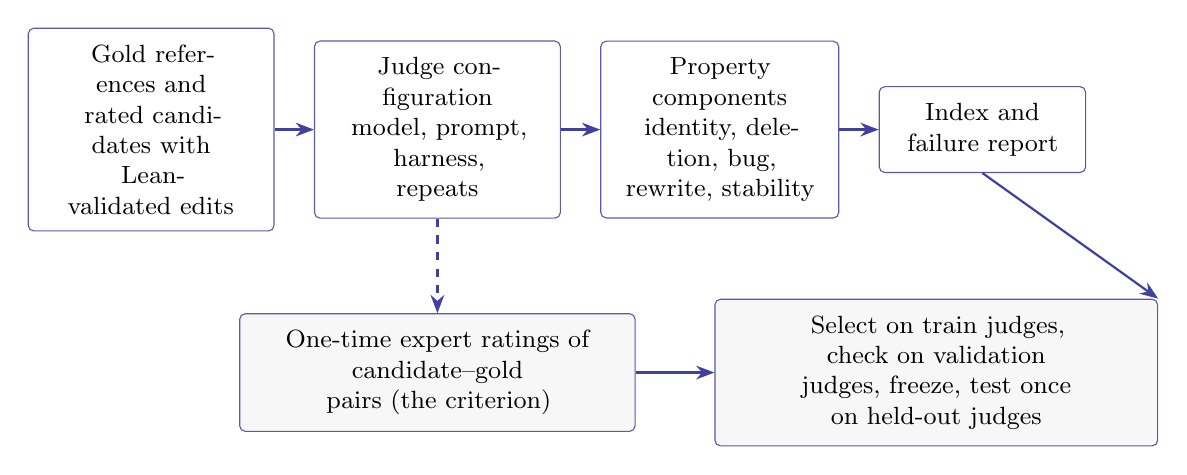
\begin{tikzpicture}[>=Stealth, node distance=5mm,
 box/.style={draw=darkblue!65,rounded corners=2pt,align=center,inner sep=6pt,font=\small},
 flow/.style={->,thick,draw=darkblue!75}]
\node[box,text width=27mm] (gold) {Gold references and\\rated candidates with\\Lean-validated edits};
\node[box,text width=27mm,right=of gold] (judge) {Judge configuration\\model, prompt, harness,\\repeats};
\node[box,text width=26mm,right=of judge] (checks) {Property components\\identity, deletion, bug,\\rewrite, stability};
\node[box,text width=22mm,right=of checks] (index) {Index and\\failure report};
\draw[flow] (gold)--(judge); \draw[flow] (judge)--(checks); \draw[flow] (checks)--(index);
\node[box,text width=46mm,below=12mm of judge,fill=gray!6] (panel) {One-time expert ratings of\\candidate--gold pairs (the criterion)};
\node[box,text width=52mm,right=10mm of panel,fill=gray!6] (select) {Select on train judges, check on validation\\judges, freeze, test once on held-out judges};
\draw[flow] (panel)--(select);
\draw[flow] (index.south)--(select.north east);
\draw[flow,dashed] (judge.south)--(panel.north);
\end{tikzpicture}
\end{adjustbox}
\caption{\textbf{Human ratings enter once (bottom); every later judge faces only the automated checks (top).} The bottom path selects the screen on the train and validation judges and evaluates the frozen choice once on judge models that neither step touched.}
\label{fig:protocol}
\end{figure}

\begin{table}[t]
\centering\small
\begin{tabularx}{\linewidth}{@{}lXX@{}}
\toprule
Stage & Human ratings & Judge computation \\
\midrule
Establish the criterion & Experts rate candidate--gold pairs once & Measure each configuration's agreement and its property components \\
Select and freeze & Use the train and validation judges' agreement & Rank the candidate family on the train judges, pick on the validation judges, seal the test rows \\
Test transfer & Do not consult the ratings again & Compute the frozen screen on the held-out judges; apply the pre-registered gates once \\
Screen a new judge & None & Run the frozen probes; inspect the index and the failure report \\
\bottomrule
\end{tabularx}
\caption{\textbf{Screening a new judge costs inference, not ratings; the transfer test is a one-shot evaluation on judges the screen was not selected on.} The split is over judge models and harnesses, not over items, because the question is whether the screen carries over to a new judge.}
\label{tab:protocol_workflow}
\end{table}

\paragraph{Probes and components.}
Every probe is a scripted edit of a gold reference $g$ or of a rated candidate $x$, and every edited file must elaborate under Lean~4.22 with Mathlib; an edit that fails to elaborate is excluded before any judge call and counted.
Ten components summarize a configuration's responses (exact definitions in Appendix~\ref{app:index-definitions}).
\emph{Identity} is the median score of each gold against itself, and \emph{blank} is one minus the score of an empty candidate.
\emph{Gold deletion monotonicity}, $C_{\mathrm{ms,gold}}$, is the component this paper selects, defined below.
\emph{Candidate deletion monotonicity} and \emph{gold bug monotonicity} apply the same ladder construction to a rated candidate and to cumulative implementation bugs in the gold.
\emph{Alpha-renaming}, \emph{proof-to-\texttt{sorry}}, and \emph{reordering} invariance are one minus the absolute score change under the rewrite, and \emph{spam non-increase} is one minus any score gain after theorem statements are appended to a candidate.
\emph{Stability} is one minus twice the population standard deviation across three repeated calls, averaged over the repeated cells.
For a deletion ladder, level $0$ is the gold as its own candidate and level $\ell$ removes a cumulative fraction $\ell/L$ of its theorem statements, last theorem first, with $L\le 4$.
The ladder quality is $(1-\rho)/2$ for the tie-aware Spearman correlation $\rho$ between level and median score; a constant ladder counts $0$.
$C_{\mathrm{ms,gold}}$ is the mean ladder quality over the 24 gold ladders, so a score that falls monotonically with every deletion gives $1$ and a constant or rising score gives $0$.
A component needs at least 80\% of its valid probes scored; otherwise it is missing rather than zero.

\paragraph{The candidate family and the selection rule.}
Twenty-two indices were pre-registered: the two indices of our earlier work, nine fixed aggregates of component subsets (geometric means, an arithmetic mean, and a minimum), and the ten single components.
The rule ranks every candidate by its Spearman association with the criterion over the 18 train configurations, breaking ties toward fewer components, keeps the top three, and selects the finalist with the highest validation association.
The test rows were sealed in a private file, and the selection was committed before any test row was read.
% Provenance: experiments/archive/39_.../results/SELECTION.json and FINALISTS.json (seal commit 86ae479201e5); the candidate family is analysis_lib.CANDIDATES.

\paragraph{Pre-registered gates.}
The selected index passes if its test Spearman association is at least $0.45$ and its one-sided permutation $p$ for a positive association is below $0.05$ (10{,}000 permutations).
Uncertainty is a 95\% percentile bootstrap over configurations (10{,}000 draws).
The outcome is inconclusive, never resolved by changing a threshold, if the criterion is not computable for more than five of the 18 test configurations or if the interval spans more than $1.2$.
We also report whether the train, validation, and test associations lie within $0.30$ of each other, and the two earlier indices on every split regardless of selection.
The permutation test rejects the absence of a positive association; it does not test that the population correlation exceeds $0.45$, so we report the interval's lower bound beside the verdict.

\paragraph{The two earlier indices.}
$\mathrm{TI}_{\mathrm{var}}$ is the geometric mean of the mean bug-ladder quality and two variance penalties, min--max normalized here over the train configurations (Equation~\ref{eq:tivar}, Appendix~\ref{app:index-definitions}).
$\mathrm{PTI}_{v0}$ is the frozen geometric mean of the identity, bug-ladder, deletion-ladder, and alpha-renaming properties with exact-zero geometric means and strict coverage, so it is undefined whenever any required probe is unscored and zero whenever any property is zero.
Both enter the family as frozen candidates and are reported on every split.

% !TEX root = main.tex
\section{Experiments}
\subsection{Data and human panel}\label{sec:data-human-protocol}\label{sec:veribench-overview}
We evaluate candidate--gold pairs from \textsc{VeriBench}~\citep{miranda2026veribench}.
One annotator supplied holistic ratings on a $0$--$5$ scale in two passes, pass1 with a stricter rubric and pass2 with a more lenient rubric.
The collection covered 75 pairs from 25 problems with three agent generations per problem.
One gold filename could not be resolved, leaving 72 analyzed pairs from 24 problems.
We report each pass and the archived averaged-label view; they are two judgments by one person, not independent annotators.
Inter-pass agreement is Spearman $0.249$, quadratic-weighted $\kappa=0.372$, and mean absolute error $0.771$ on the shared pairs (Appendix~\ref{app:exp16-exp17}).
These statistics describe label disagreement; they do not establish an upper bound on judge agreement.
The original written rubric was not recovered, so we cannot reconstruct every annotation instruction.

This panel is the \emph{validation set}: it informed index-form selection, repeat aggregation, the threshold, and the prompt panel, so correlations on it are optimistic.
The fixed equal-weight $\mathrm{TI}_{\mathrm{var}}$ has no training set.
A separate weight-tuned comparison uses these same pairs, and no analysis constitutes a test-set result.
For each judge, artifact-level agreement is the Spearman correlation between its scores and the human ratings on the same analyzed pairs.
We then ask whether the index orders configurations by that agreement.

\subsection{Property checks on GPT-5.3-Codex}\label{sec:property-results}
Figure~\ref{fig:judge_sanity_checks} summarizes the 24-problem panel for three Codex prompts.
Their mean scores decrease as bug-ladder edits accumulate, but averages conceal local reversals.
The strict prompt reverses on four of 24 ladders, whereas the baseline and checklist prompts have no reversals (Table~\ref{tab:codex_configs}).
The archived alpha probes produce the largest score changes among the four rewrite types, but their generator can produce malformed Lean text.
The baseline and checklist prompts assign them zero mean score, despite near-maximum scores for the other rewrites.
The strict prompt gives alpha-renamed artifacts a mean score of $0.179$.
Appendix~\ref{app:failure-diagnostics} retains the per-configuration diagnostics and the corresponding Claude Opus summary.

\begin{figure}[t]
\centering
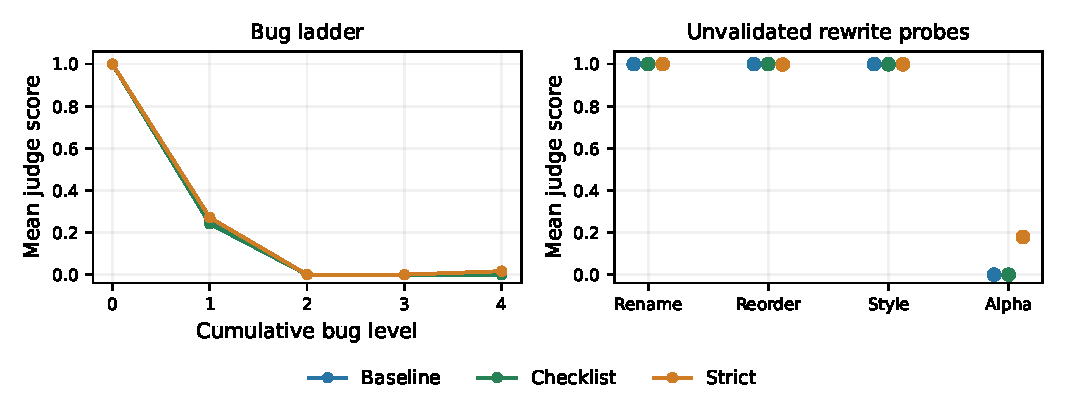
\includegraphics[width=\linewidth]{figures/codex_property_checks.pdf}
\caption{Mean scores fall with cumulative bug edits, but malformed alpha probes sharply change the Codex judges' scores.
Each point averages median scores over 24 problems, with three calls per problem and prompt; these are descriptive means, not uncertainty intervals.
Local reversals remain visible in Table~\ref{tab:codex_configs}.}
\label{fig:judge_sanity_checks}
\end{figure}

\paragraph{Alpha-renaming and a canonicalization proxy.}
The historical alpha routine can duplicate the assignment marker and rename signature variables without updating the proof body.
Its score drops therefore cannot establish a failure of invariance under valid alpha-renaming.
A post-hoc proxy replaces each judge's alpha scores with its median score under style edits.
Across the eight Codex-panel configurations, this lowers the mean per-judge standard deviation across identity-probe scores from $0.250$ to $0.070$.
This manipulation changes recorded scores rather than the judge's inputs.
A real fix must rescore canonicalized text and verify that the transformation preserves meaning.

\paragraph{Coverage of P3.}
The eight-configuration panel contains identity rewrites and bug ladders but no missing-specification ladders.
Consequently, it cannot establish which association P3 has with human agreement.
We retain P3 as a proposed part of the protocol, without attributing the bug-ladder statistics below to it.

\subsection{The index tracks judge-level human agreement on the validation set}\label{sec:tivar_cross_model_results}\label{sec:validation-human-alignment}
The three primary families are GPT-5.3-Codex, Claude Opus 4.7, and Qwen3-Coder.
Each eight-configuration panel contains three semantic prompts, a deliberately lexical prompt on the same model, two GPT-4o-mini prompts, edit distance, and a random control.
These are family panels with shared controls, not eight independent models per family.
The frozen model identifiers and complete main-panel prompts appear in Appendix~\ref{app:judge-prompts}.
Scores are medians over three repeated calls for language-model judges; Codex-panel controls use nine repeats, and the other panels use three.

Figure~\ref{fig:tivar_cross_model_avg} uses the fixed equal-weight index in Equation~\ref{eq:tivar}.
Its judge-level Spearman association is positive for each primary family and label view (Table~\ref{tab:tivar_cross_model_results}).
For Codex, averaged-label Pearson and Kendall associations are $0.868$ and $0.643$, respectively.
The Codex bootstrap intervals are wide, and the resampling does not correct for the earlier protocol selection.
Pass-to-pass differences also matter: Qwen's Spearman association changes from $0.476$ on pass1 to $0.857$ on pass2.
With eight configurations and disagreeing label passes, these estimates support a descriptive association rather than a precise or portable effect size.

\begin{figure}[t]
\centering
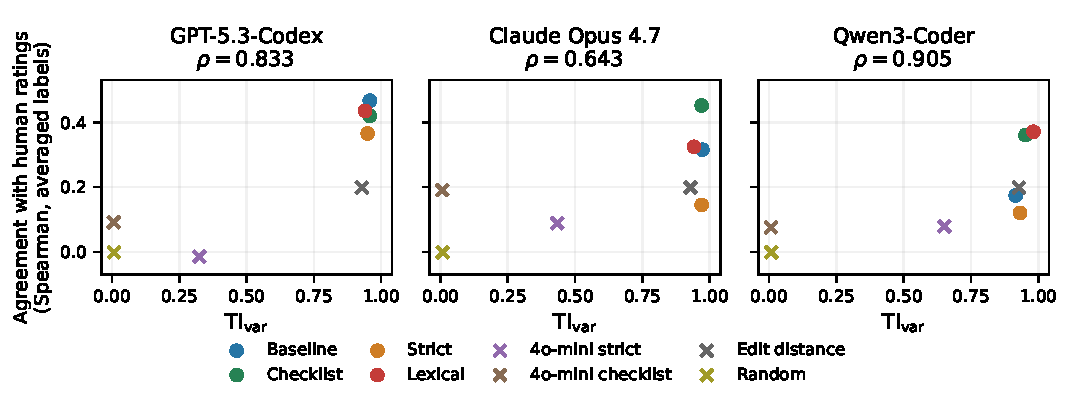
\includegraphics[width=\linewidth]{figures/judge_agreement_fixed_index.pdf}
\caption{The fixed equal-weight index has a positive association with human agreement in each primary family, but high index values do not rule out lexical judges.
Each point is one configuration; the vertical axis is its Spearman agreement with averaged human labels on 72 pairs.
Panel titles report the correlation across eight configurations; Table~\ref{tab:tivar_cross_model_results} gives Codex uncertainty.}
\label{fig:tivar_cross_model_avg}
\end{figure}

\begin{table}[t]
\centering\small
\begin{tabular}{@{}lrrrrrr@{}}
\toprule
& \multicolumn{4}{c}{Averaged labels} & \multicolumn{2}{c}{$\mathrm{TI}_{\mathrm{var}}$ by pass} \\
\cmidrule(lr){2-5}\cmidrule(lr){6-7}
Family & $v1$ & $v2$ & $\mathrm{GM}_{.4,.6}$ & $\mathrm{TI}_{\mathrm{var}}$ & pass1 & pass2 \\
\midrule
Codex & 0.762 & 0.476 & 0.857 & 0.833 & 0.905 & 0.738 \\
Claude Opus & 0.429 & 0.143 & 0.714 & 0.643 & 0.810 & 0.595 \\
Qwen3-Coder & 0.524 & 0.500 & 0.786 & 0.905 & 0.476 & 0.857 \\
\midrule
\multicolumn{4}{l}{Codex $\mathrm{TI}_{\mathrm{var}}$: 95\% interval} & $[0.24,1.00]$ & $[0.41,1.00]$ & $[0.11,1.00]$ \\
\multicolumn{4}{l}{Codex $\mathrm{TI}_{\mathrm{var}}$: permutation $p$} & 0.017 & 0.005 & 0.045 \\
\bottomrule
\end{tabular}
\caption{The fixed index is competitive with a two-component geometric comparison whose weights were selected on pass1.
Entries are Spearman correlations between each index and judge-level human agreement on the validation set, with eight configurations per family.
Codex intervals and permutation probabilities use 10{,}000 resamples and permutations, seed 42; corresponding intervals for the other families are not reported.
Appendix~\ref{app:index-definitions} defines all indices.}
\label{tab:tivar_cross_model_results}\label{tab:cross_model_index_compare_avg}
\end{table}

\paragraph{Human agreement alone can miss a bad judge.}
The lexical prompt, \texttt{BAD\_STRINGY}, explicitly instructs the model to ignore theorem meaning and grade textual overlap.
On the Codex panel, its human agreement of $0.435$ lies among the semantic prompts' values, $0.365$--$0.466$.
Yet it reverses on 20 of 24 bug ladders (Table~\ref{tab:codex_configs}).
The index ranks it below the three semantic prompts, but its value remains $0.940$; edit distance also scores highly at $0.928$.
In the Qwen panel, the lexical configuration has the highest index value, $0.982$.
The failure report therefore carries information that both human agreement and the scalar can miss.
No validated cutoff on $\mathrm{TI}_{\mathrm{var}}$ establishes that a judge is acceptable.

\begin{table}[t]
\centering\small
\begin{tabular}{@{}lrrr@{}}
\toprule
Codex-panel configuration & Human $\rho$ (avg) & $\mathrm{TI}_{\mathrm{var}}$ & Ladders with reversals \\
\midrule
Baseline prompt & 0.466 & 0.958 & 0/24 \\
Checklist prompt & 0.419 & 0.958 & 0/24 \\
Strict prompt & 0.365 & 0.950 & 4/24 \\
Lexical prompt & 0.435 & 0.940 & 20/24 \\
GPT-4o-mini, strict & $-0.014$ & 0.324 & 18/24 \\
GPT-4o-mini, checklist & 0.092 & 0.007 & 16/24 \\
Edit distance & 0.199 & 0.928 & 24/24 \\
Random & $-0.001$ & 0.008 & 24/24 \\
\bottomrule
\end{tabular}
\caption{The lexical judge agrees with humans despite frequent bug-ladder reversals, and the scalar index penalizes it only slightly.
A reversal is any local score increase as cumulative edits are added; the diagnostic uses the recorded repeat-aggregated scores.}
\label{tab:codex_configs}
\end{table}

\paragraph{Choice of index.}
The two-component geometric comparison is numerically higher than $\mathrm{TI}_{\mathrm{var}}$ for Codex and Opus on averaged labels (Table~\ref{tab:tivar_cross_model_results}).
It uses bug monotonicity and decision stability with weights $0.4$ and $0.6$, selected on pass1, rather than fixed equal weights.
We retain $\mathrm{TI}_{\mathrm{var}}$ for its explicit variance penalties and positive associations across the primary families and passes, not because these data establish its superiority.
A separate search over six component weights gives cross-pass associations of $0.810$ and $0.786$ on the same pairs (Appendix~\ref{app:moved-results}).
The pass1-selected geometric form reaches $0.769$ on an expanded 13-configuration panel, with a 95\% interval of $[0.34,0.95]$ (Appendix~\ref{app:expanded-panel}).
Neither comparison provides a held-out estimate.
A separate Leanstral panel has averaged-label association $-0.095$ for the fixed index (Appendix~\ref{app:negative-results}), so the positive result does not hold for every recorded family.

\paragraph{Weight and normalization sensitivity.}
Recomputing the fixed index on a local grid of weight triples gives averaged-label Spearman ranges of $0.738$--$0.857$ for Codex, $0.643$--$0.714$ for Opus, and $0.881$--$0.976$ for Qwen.
This analysis uses only committed component vectors and keeps their normalization fixed (Appendix~\ref{app:weight-sensitivity}).
It does not assess sensitivity to changing the normalization panel.
We do not report leave-one-family-out transfer: the panels share controls and normalize separately, so pooling their scores would not constitute an independent family test.

\paragraph{Which measured statistics matter.}
Among the recorded diagnostics, weak monotonicity on bug ladders has the largest association with human agreement on each label view (Table~\ref{tab:property_assoc}).
It measures the absence of local increases; bug-rank correlation measures the overall direction.
The archived field name \texttt{P3\_weak\_mono} refers to this bug statistic, not to the P3 missing-specification property.
Identity-rewrite scores and repeat decision stability have weaker or inconsistent associations.
Only the weak-monotonicity statistic on pass2 and averaged labels has an unadjusted permutation $p<0.05$; these component comparisons are exploratory.

\begin{table}[t]
\centering\small
\begin{tabular}{@{}lrrr@{}}
\toprule
Measured diagnostic & pass1 & pass2 & avg \\
\midrule
Mean identity-rewrite score & $-0.21$ (0.62) & 0.02 (0.98) & $-0.02$ (0.98) \\
Bug-rank monotonicity & 0.60 (0.13) & 0.67 (0.08) & 0.71 (0.06) \\
Bug weak monotonicity & 0.63 (0.11) & 0.78 (0.03) & 0.75 (0.04) \\
Repeat decision stability & 0.47 (0.24) & $-0.23$ (0.57) & 0.14 (0.76) \\
\bottomrule
\end{tabular}
\caption{Bug weak monotonicity has the largest observed association among the measured diagnostics; this table contains no P3 missing-specification result.
Entries are Spearman correlations with human agreement across eight Codex-panel configurations; unadjusted permutation probabilities appear in parentheses.}
\label{tab:property_assoc}
\end{table}

\paragraph{Artifact-score threshold.}
A historical sweep of the artifact-score threshold from $0.60$ to $0.85$ lowers the observed decision-flip rate from $0.058$ to $0.046$ and pass rate from $0.583$ to $0.536$ (Appendix Table~\ref{tab:exp13_threshold_sweep}).
The selected threshold is $0.85$, which has the lowest observed flip rate in that sweep.
This thresholds $J_\theta(x,g)$, not the judge-level index, and measures repeatability rather than correctness of the accepted artifacts.

% !TEX root = main.tex
\section{Limitations and Held-Out Test Protocol}\label{sec:limitations-test}
\paragraph{Validation set, not a test set.}
The same human labels informed the index form, repeat aggregation, threshold, and prompt panel, so Section~\ref{sec:validation-human-alignment} reports validation-set associations, not out-of-sample estimates.
The panel is small (72 analyzed pairs, one annotator, eight configurations per family), and its two rating passes agree only moderately.
We also collected 343 labels from five raters over 78 candidate--gold pairs, which the validation-set results do not use.
That pool was rated under a different rubric (statement coverage with a spam deduction) and correlates only weakly with the panel labels (Spearman \(\approx0.13\) on 63 shared pairs), so it measures a different criterion rather than offering a held-out test of the same one.
Two pre-registered screens nevertheless asked whether any label-free property signal tracks judge alignment with that pool.
A first pass over 14 configurations was underpowered, and an expanded pass over 32 configurations found no index meeting its registered bar (strongest Spearman \(-0.39\), Holm-adjusted permutation \(p=0.25\); leave-one-out selection transfer \(\rho=0.24\), \(p=0.49\)).
A locked held-out test therefore needs independent raters under one frozen rubric, with the properties and \(\mathrm{TI}_{\mathrm{var}}\) fixed in advance.

\paragraph{What certification does not cover.}\label{sec:limitations-finite}
No finite perturbation suite can rule out every judge failure, so \(\mathrm{TI}_{\mathrm{var}}\) is a graded trust signal, not a pass/fail certificate.
The four probes do not target vacuous, weakened, or over-constrained statements, formatting-only edits beyond the rewrites in Table~\ref{tab:codex_invariance_variants}, or artifacts from proof assistants other than Lean~4.
Scores are specification-relative: they measure agreement with an audited but necessarily incomplete gold reference, since no algorithm decides specification equivalence in general~\citep{rice1953}.
Scores are anchored to a gold reference, but we do not evaluate candidates optimized against the judge, so resistance to gaming remains untested.
Neither the judge prompts nor the validation-set rating protocol explicitly addresses presentation aspects of specification quality, such as redundant theorem statements, oversized implementations, or needless abstraction; only the held-out reviewer pool's rubric deducts for superfluous theorem statements.
Holistic panel ratings may reflect these aspects implicitly, but we did not measure this; future rating protocols should make them explicit.


% !TEX root = main.tex
\section{Conclusion}
A one-time human panel can support a protocol that screens new judges through falsifiable behavioral checks without collecting labels for each configuration.
On the present validation set, the fixed equal-weight index is associated with human agreement, but its high scores can coexist with lexical failures.
Individual property diagnostics therefore remain essential, and a locked test must establish transfer beyond the labels used to select the protocol.
The goal is to make human judgment a reusable foundation for checking new judges, with each judge accountable to explicit tests of its behavior.

% !TEX root = main.tex
\clearpage
\section*{Reproducibility Statement}
The accompanying repository preserves frozen scores and summaries under \path{experiments/archive/}.
Appendix~\ref{app:judge-prompts} gives the prompt templates, exact model identifiers, input extraction, and repeat aggregation used for the main panels.
Appendix~\ref{app:index-definitions} specifies the indices, including normalization and numerical edge cases.
The manuscript evidence script, \path{experiments/34_iclr_mega_rewrite_astra/analysis/rebuild_paper_evidence.py}, reads committed artifacts, verifies their hashes, and regenerates the corrected figures and sensitivity summaries without inference.
Its output manifest maps every input to a repository path and content hash.
The adjacent report maps every reported table to the archived script and machine-readable output that produced it.
The original human-panel rubric text was not recovered, which limits exact replication of the annotation process.
We describe repository paths without an identifying repository URL for anonymous review.

\section*{Ethics Statement}
An author supplied the human ratings used for the headline validation analysis.
The study evaluates generated Lean code and formal statements, without personal data in the judged artifacts.
It makes no deployment claim and does not establish that screened judges can replace expert review in consequential settings.

\section*{LLM Usage Statement}
% TODO(Brando): confirm the factual scope of writing/editing assistance and author supervision before submission.
LLMs served as the judges under study and assisted with writing and editing under author supervision.
The authors are responsible for the manuscript's claims, citations, and interpretation of the recorded results.

% References
\bibliographystyle{iclr2027_conference}
\bibliography{refs} % expects refs.bib in the same directory


\clearpage
\appendix
% !TEX root = main.tex
\section{Judge Prompts and Scoring Configuration}\label{app:judge-prompts}
\paragraph{Judges and prompts of the transfer study (Section~\ref{sec:setup}).}
% Provenance: experiments/archive/39_label_free_proxy_index_train_val_test_over_judge_families/scripts/e39.py (MODELS, PROMPTS) and results.md ("Selectors actually used").
The six judge models were served through one hosted gateway under the identifiers \texttt{openai/gpt-6-sol-high} (reasoning effort high), \texttt{anthropic/claude-sonnet-5-medium} (compute effort medium), \texttt{openai/gpt-6-luna-high} (high), \texttt{google/gemini-3.1-pro-preview}, \texttt{anthropic/claude-opus-5-5-no-fallback} (compute effort maximum), and \texttt{alibaba/qwen3.6-27b}.
The agent judges ran the same models inside the Terminus2 harness (at most 20 turns, reasoning effort high where exposed) and wrote their verdict to a file.
The five fuller-context prompts are \textsc{VeriBench}'s frozen rubrics, imported byte-for-byte: \texttt{D0\_deployed\_tc\_v1} (integer $0$--$10$, divided by ten), \texttt{R4\_exp75\_human\_precondition}, \texttt{H0\_human\_mirror}, \texttt{H1\_human\_mirror\_rater\_conventions}, and \texttt{H2\_human\_mirror\_conventions\_demos} (integer $0$--$5$, divided by five); each shows the judge the complete reference, the task's Python source, and the full candidate.
The four legacy prompts are the \texttt{P1\_BASELINE}, \texttt{P4\_CHECKLIST}, \texttt{P8\_STRICT\_B}, and \texttt{BAD\_STRINGY} prompts listed below, verbatim, with the reference field holding the gold's last theorem block as in our earlier version.
Scores were normalized to $[0,1]$ at parse time, and the expert target is the $0$--$5$ mean divided by five, so no further scaling is applied.

\paragraph{Prompts of the earlier 72-pair validation set (Appendix~\ref{app:validation-set-72}).}
The primary family model identifiers are \texttt{gpt-5.3-codex}, \texttt{claude-opus-4-7}, and \texttt{Qwen/Qwen3-Coder-30B-A3B-Instruct}.
Each family panel contains the three semantic prompts below and \texttt{BAD\_STRINGY}, plus \texttt{gpt-4o-mini} with the checklist and strict prompts.
The other two configurations are the deterministic edit-distance control \texttt{editdist\_e1} and seeded control \texttt{random\_r1}.
All model prompts request scores in $[0,1]$, not integers on a $0$--$10$ scale.
The human ratings use $0$--$5$; correlations compare their ordering with judge scores without equating the scales.

The reference field retains its historical label ``REFERENCE IMPLEMENTATION,'' but the code fills it with the gold's final theorem block.
The candidate field contains the full candidate file for human-agreement scoring; property probes operate on the extracted theorem text.
If no theorem block is found, the extractor uses the full file.
The Codex panel aggregates three recorded calls for model configurations and nine for controls by the median.
The Opus and Qwen panels aggregate three calls for every configuration by the median.
These counts come from the saved repeat arrays; a summary-level repeat setting alone does not describe reused cached rows.
The random control is deterministic for its input and seed, so repeated identical scores do not imply a reliable semantic judge.
Prompt labels P1, P4, and P8 are historical identifiers and do not denote the property numbers P1--P4.

\noindent\textbf{\texttt{P1\_BASELINE}}\par
\vspace{0.25em}\begin{lstlisting}[style=promptstyle]
You are an expert in Lean 4 formal verification.
Score how well the GENERATED THEOREM captures the correctness properties
of the REFERENCE IMPLEMENTATION. Score from 0.0 to 1.0.

- 1.0: Semantically equivalent to what the reference guarantees
- 0.7-0.9: Captures most properties, misses minor ones
- 0.4-0.6: Captures some properties, has meaningful gaps
- 0.1-0.3: Technically valid Lean but misses core properties
- 0.0: Trivially true (e.g., `True`) or incorrect

REFERENCE IMPLEMENTATION:
{reference_impl}

GENERATED THEOREM:
{generated_theorem}

Respond ONLY with valid JSON, no markdown:
{"score": <float 0.0-1.0>,
 "reasoning": "<one sentence max>"}
\end{lstlisting}

\noindent\textbf{\texttt{P4\_CHECKLIST}}\par
\vspace{0.25em}
\begin{lstlisting}[style=promptstyle]
Evaluate this in order:
1) What properties does REFERENCE IMPLEMENTATION guarantee?
2) Which are preserved by GENERATED THEOREM?
3) Are there missing core guarantees or trivialization?
4) Map to score in [0.0, 1.0]:
   1.0 equivalent; 0.7-0.9 minor gaps;
   0.4-0.6 meaningful gaps; 0.1-0.3 weak;
   0.0 trivial/incorrect.

REFERENCE IMPLEMENTATION:
{reference_impl}

GENERATED THEOREM:
{generated_theorem}

Return JSON only:
{"score": <float 0.0-1.0>,
 "reasoning": "<one sentence>"}
\end{lstlisting}

\noindent\textbf{\texttt{P8\_STRICT\_B}}\par
\vspace{0.25em}
\begin{lstlisting}[style=promptstyle]
Evaluate conservatively. If uncertain, choose the lower score.
Use [0.0,1.0]:
1.0 equivalent semantics
0.7-0.9 mostly right, minor misses
0.4-0.6 substantial omissions
0.1-0.3 weak relation
0.0 trivial/incorrect

REFERENCE IMPLEMENTATION:
{reference_impl}

GENERATED THEOREM:
{generated_theorem}

Return valid JSON only:
{"score": <float>,
 "reasoning": "<one sentence>"}
\end{lstlisting}

\noindent\textbf{\texttt{BAD\_STRINGY negative control}}\par
\vspace{0.25em}
\begin{lstlisting}[style=promptstyle]
You are a text similarity grader.
Compare generated theorem text to the reference implementation text.
Do NOT evaluate semantic correctness or theorem meaning.
Score ONLY based on superficial lexical/format overlap:
- high score if tokens/phrases look similar
- low score if wording/structure differs
Reference implementation:
{reference_impl}

Generated theorem:
{generated_theorem}

Return ONLY a JSON object:
{"score": <float 0.0 to 1.0>,
 "reasoning": "<short reason>"}
\end{lstlisting}



% !TEX root = main.tex
\section{Index Definitions and Implementation}\label{app:index-definitions}
\paragraph{Fixed equal-weight index.}
For each file $f$ and bug level $\ell$, let $s_{f\ell}$ be the median recorded repeat score and $v_{f\ell}$ its population variance.
Let $\rho_f$ be Spearman's correlation between level and $s_{f\ell}$, and set $c_f=\mathrm{clip}((1-\rho_f)/2,0,1)$.
Writing $\mathcal F$ for the included ladders, the archived implementation uses
\[
 C_f=\frac1{|\mathcal F|}\sum_{f\in\mathcal F}c_f,\qquad
 V_c=\mathrm{Var}_{f\in\mathcal F}(c_f),\qquad
 V_s=\frac{\sum_{f\in\mathcal F}\sum_\ell v_{f\ell}}{\sum_{f\in\mathcal F}L_f},
\]
where $L_f$ is the number of levels in ladder $f$.
It skips ladders with fewer than three levels or an undefined Spearman correlation, including constant-score ladders.
All primary committed vectors report 24 included ladders per configuration.
If none remain, the code substitutes $C_f=0$, $V_c=1$, and $V_s=1$.
It min--max normalizes each variance across the current family panel; a constant variance column maps to zero.
Equation~\ref{eq:tivar} then applies weights $1/3$ to $C_f$, $1-\widetilde V_c$, and $1-\widetilde V_s$, after clipping each to $[10^{-6},1]$.
Thus an extreme variance does not produce an exact zero index, and adding a judge can change other judges' normalized scores.
The analysis preserves these choices rather than changing the frozen index after observing results.

\paragraph{Arithmetic comparisons.}
The recorded $v1$ and $v2$ are
\[
 v1=0.30\,\mathrm{ident}+0.30\,\mathrm{mono}+0.25\,\mathrm{weak}+0.15\,\mathrm{stab},
\]
\[
 v2=0.20\,\mathrm{ident}+0.20\,\mathrm{mono}+0.15\,\mathrm{weak}+0.10\,\mathrm{stab}+0.20\,\mathrm{anti}+0.15\,\mathrm{subtle}.
\]
Here $\mathrm{ident}$ is mean score over identity-rewrite probes, $\mathrm{mono}=(1-\rho_{\mathrm{bug}})/2$ uses the pooled bug-level Spearman correlation, and $\mathrm{weak}$ is the weak-monotonicity fraction on bug ladders.
The latter is the historical field \texttt{P3\_weak\_mono}; it contains no missing-specification measurement.
$\mathrm{stab}$ is one minus the fraction of scored pairs whose repeated scores cross the artifact-score threshold.
$\mathrm{anti}$ is the complement of the absolute score correlation with normalized edit distance, clipped to $[0,1]$, and $\mathrm{subtle}$ is the clipped mean first-level score drop divided by $0.25$.
The implementation clips these components to $[0,1]$.
These arithmetic indices combine different summaries from $\mathrm{TI}_{\mathrm{var}}$ and do not isolate the effect of changing only the aggregation function.

\paragraph{Geometric comparisons.}
The two-component comparison in Table~\ref{tab:tivar_cross_model_results} is $\mathrm{GM}_{.4,.6}=\mathrm{mono}^{0.4}\mathrm{stab}^{0.6}$, with the same $10^{-6}$ component floor.
Its weights originate in the pass1 search over six components; it is not a fixed equal-weight baseline.
The separate cross-pass analysis searches nonnegative weights summing to one over $\mathrm{ident}$, $\mathrm{mono}$, $\mathrm{weak}$, $\mathrm{stab}$, $\mathrm{anti}$, and $\mathrm{subtle}$.
Table~\ref{tab:cross_pass_generalization} identifies which pass supplies those fitted weights.
Neither procedure fits the weights of $\mathrm{TI}_{\mathrm{var}}$.

% !TEX root = main.tex
\section{The Earlier 72-Pair Validation Set: Results, Provenance, and Selection Bias}\label{app:validation-set-72}
% TLDR: the validation-set results that the earlier version of this paper reported in its main text, moved here with the provenance audit (experiment 41) and the best-of-k selection-bias analysis (experiment 40) that qualify them. Framing decided 10-13-2026 (docs/PAPER_FRAMING_DECISION_10-13-2026.md).
Our earlier version selected and evaluated $\mathrm{TI}_{\mathrm{var}}$ on one 72-pair panel.
The numbers below reproduce to three decimals from the frozen score vectors, and we keep them because they motivated the transfer study; the two subsections that follow them record why they are not evidence of transfer.

\subsection{The validation set}\label{sec:data-human-protocol}\label{sec:veribench-overview}
% Provenance: experiments/archive/41_paper_panel_provenance_audit_and_vb_expert_label_rescore/REPORT.md ("Label identity", "Judge-seen vs. rater-seen references"); Appendix app:exp16-exp17 for the inter-pass statistics.
We evaluated candidate--gold pairs from \textsc{VeriBench}~\citep{miranda2026veribench}.
One rater supplied holistic ratings on a $0$--$5$ scale in two passes, pass1 under a stricter rubric and pass2 under a more lenient one.
The collection covered 75 pairs from 25 problems with three agent generations per problem.
One gold filename could not be resolved by the frozen judge pipeline, leaving 72 analyzed pairs from 24 problems.
We report each pass and the archived averaged-rating view; they are two ratings by one person, not independent raters.
Inter-pass agreement is Spearman $0.249$, quadratic-weighted $\kappa=0.372$, and mean absolute error $0.771$ on the shared pairs (Appendix~\ref{app:exp16-exp17}).
This panel is a \emph{validation set}: it informed index-form selection, repeat aggregation, the threshold, and the prompt panel, so correlations on it are optimistic.
$\mathrm{TI}_{\mathrm{var}}$ has no fitted weights, so there is no training set, and no analysis on this panel is a test-set result.
For each judge, artifact-level agreement is the Spearman correlation between its scores and the human ratings on the analyzed pairs.

\subsection{Property checks on GPT-5.3-Codex}\label{sec:property-results}
Figure~\ref{fig:judge_sanity_checks} summarizes the 24-problem panel for the three semantic Codex prompts.
Each bug ladder has five levels, the original artifact plus four cumulative edits, and each artifact has four rewrite probes.
Mean scores fall from $1.0$ at level zero to $0.24$--$0.27$ after the first cumulative edit and to about zero thereafter.
Averages conceal local reversals: the strict prompt reverses on four of 24 ladders, whereas the baseline and checklist prompts have none (Table~\ref{tab:codex_configs}).
Renaming, reordering, and style rewrites leave mean scores at or near $1.0$.
The archived alpha probes are the exception, but their generator can produce malformed Lean text; the baseline and checklist prompts assign them a mean score of zero and the strict prompt $0.179$.
These historical probes were string edits without Lean elaboration, unlike the probes of Section~\ref{sec:setup}; Appendix~\ref{app:failure-diagnostics} records their limitations.
The eight-configuration panels contain rewrite probes and bug ladders but no deletion ladders, so they cannot speak to the component that transferred.

\begin{figure}[htbp]
\centering
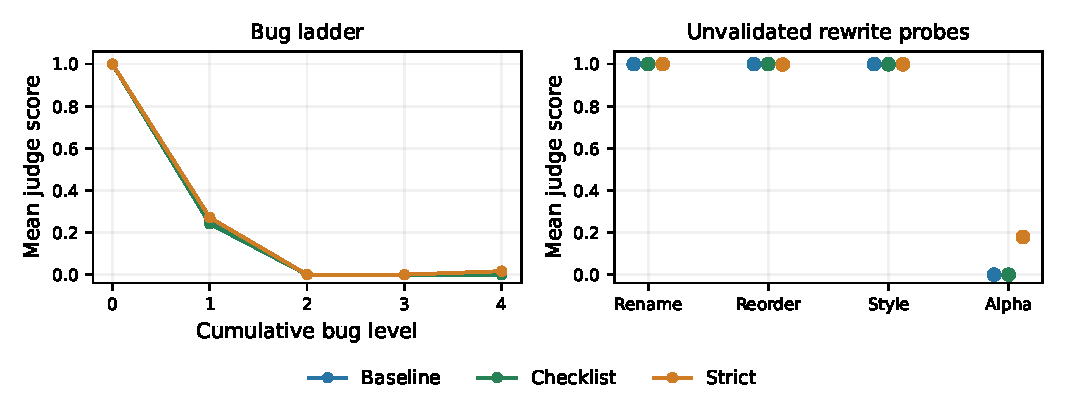
\includegraphics[width=\linewidth]{figures/codex_property_checks.pdf}
\caption{\textbf{Early bug edits and malformed alpha probes lower the Codex judges' mean scores.} Each point averages median scores over 24 problems, with three calls per problem and prompt; these are descriptive means, not uncertainty intervals.
Local reversals remain visible in Table~\ref{tab:codex_configs}.}
\label{fig:judge_sanity_checks}
\end{figure}

\subsection{The index tracks judge-level human agreement on the validation set}\label{sec:tivar_cross_model_results}\label{sec:validation-human-alignment}
% Provenance: experiments/archive/41_.../REPORT.md gate G0 (reproduces 0.833 / 0.905 / 0.738 and the Opus and Qwen rows to three decimals); experiments/archive/38_iclr_body_rewrite_to_trust_artifact_abstract/analysis/results/judge_level_diagnostics.csv.
The three primary families are GPT-5.3-Codex, Claude Opus 4.7, and Qwen3-Coder.
Each eight-configuration panel contains three semantic prompts, a deliberately lexical prompt on the same model, two GPT-4o-mini prompts, edit distance, and a random control.
These are family panels with shared controls, not eight independent models per family.
Scores are medians over three repeated calls for language-model judges; the Codex-panel controls use nine repeats, and the other panels use three.
Figure~\ref{fig:tivar_cross_model_avg} uses the fixed equal-weight index of Equation~\ref{eq:tivar}, normalized within each family panel.
Its judge-level Spearman association is positive for each primary family and rating view (Table~\ref{tab:tivar_cross_model_results}).
For Codex, the averaged-rating Pearson and Kendall associations are $0.868$ and $0.643$.
Exact permutation probabilities over all $8!$ orderings are $0.096$, $0.022$, and $0.132$ for Claude Opus and $0.005$, $0.243$, and $0.011$ for Qwen3-Coder on averaged, pass1, and pass2 ratings (Appendix~\ref{app:judge-level-diagnostics}).
Only some cells are individually distinguishable from a random ordering at the $0.05$ level, and the nine tests are unadjusted.
Excluding random, edit distance, and the lexical prompt leaves five semantic configurations, with averaged-rating associations of $0.900$ for Codex, $0.600$ for Claude Opus, and $0.900$ for Qwen3-Coder.
A separate Leanstral panel has averaged-rating association $-0.095$ (Appendix~\ref{app:negative-results}), so the positive result did not hold for every recorded family even on this panel.
On the held-out judges of Section~\ref{sec:transfer}, the same index normalized on the train configurations has association $-0.332$.

\begin{figure}[htbp]
\centering
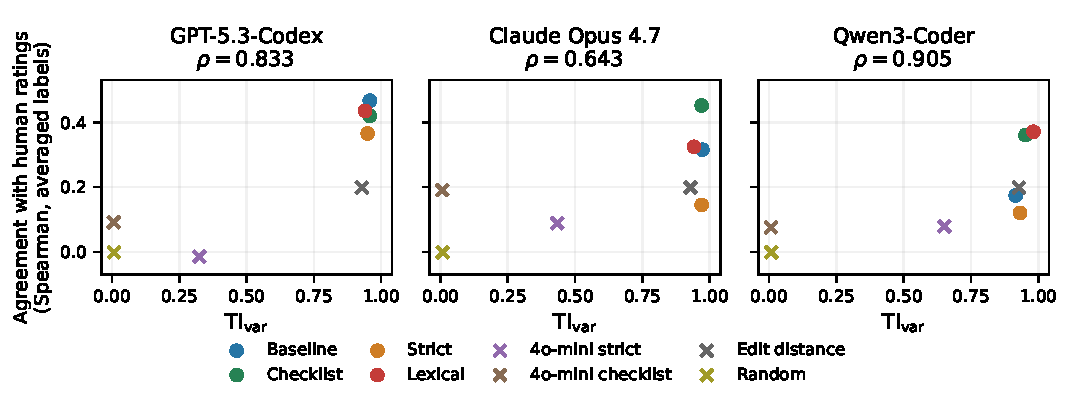
\includegraphics[width=\linewidth]{figures/judge_agreement_fixed_index.pdf}
\caption{\textbf{On the validation set the fixed equal-weight index has a positive association with human agreement in each primary family, but high index values do not rule out lexical judges.} Each point is one configuration; the vertical axis is its Spearman agreement with averaged human ratings on 72 pairs.
Panel titles report the correlation across eight configurations; Table~\ref{tab:tivar_cross_model_results} gives Codex uncertainty.}
\label{fig:tivar_cross_model_avg}
\end{figure}

\begin{table}[htbp]
\centering\small
\begin{tabular}{@{}lrrrrrr@{}}
\toprule
& \multicolumn{4}{c}{Averaged ratings} & \multicolumn{2}{c}{$\mathrm{TI}_{\mathrm{var}}$ by pass} \\
\cmidrule(lr){2-5}\cmidrule(lr){6-7}
Family & $v1$ & $v2$ & $\mathrm{GM}_{.4,.6}$ & $\mathrm{TI}_{\mathrm{var}}$ & pass1 & pass2 \\
\midrule
Codex & 0.762 & 0.476 & 0.857 & 0.833 & 0.905 & 0.738 \\
Claude Opus & 0.429 & 0.143 & 0.714 & 0.643 & 0.810 & 0.595 \\
Qwen3-Coder & 0.524 & 0.500 & 0.786 & 0.905 & 0.476 & 0.857 \\
\midrule
\multicolumn{4}{l}{Codex $\mathrm{TI}_{\mathrm{var}}$: 95\% interval} & $[0.24,1.00]$ & $[0.41,1.00]$ & $[0.11,1.00]$ \\
\multicolumn{4}{l}{Codex $\mathrm{TI}_{\mathrm{var}}$: permutation $p$} & 0.017 & 0.005 & 0.045 \\
\bottomrule
\end{tabular}
\caption{\textbf{On the validation set the fixed index is competitive with a two-component geometric comparison whose weights were selected on pass1.} Entries are Spearman correlations between each index and judge-level human agreement, with eight configurations per family.
Codex intervals and permutation probabilities use 10{,}000 resamples and permutations, seed 42; exact permutation probabilities for every cell are in Appendix~\ref{app:judge-level-diagnostics}.
Appendix~\ref{app:index-definitions} defines all indices.}
\label{tab:tivar_cross_model_results}\label{tab:cross_model_index_compare_avg}
\end{table}

\subsection{Human agreement alone can miss a bad judge}\label{sec:lexical-judge}
The lexical prompt, \texttt{BAD\_STRINGY}, instructs the model to ignore theorem meaning and grade textual overlap.
On the Codex panel, its human agreement of $0.435$ lies among the semantic prompts' values, $0.365$--$0.466$.
A validation protocol that stops at human agreement would accept it.
Yet it reverses on 20 of 24 bug ladders (Table~\ref{tab:codex_configs}).
The scalar does not expose it either: its index value is $0.940$, below the three semantic prompts but far above the failing GPT-4o-mini configurations, and edit distance scores $0.928$.
In the Qwen panel, the lexical configuration even has the highest index value, $0.982$.
The failure report therefore carries information that both human agreement and the scalar can miss, which is why the transfer study keeps the per-component report beside any index.
The same prompt is the lexical configuration of the transfer study, where it anchors the low end of both axes in Figure~\ref{fig:transfer}.

\begin{table}[htbp]
\centering\small
\begin{tabular}{@{}lrrr@{}}
\toprule
Codex-panel configuration & Human $\rho$ (avg) & $\mathrm{TI}_{\mathrm{var}}$ & Ladders with reversals \\
\midrule
Baseline prompt & 0.466 & 0.958 & 0/24 \\
Checklist prompt & 0.419 & 0.958 & 0/24 \\
Strict prompt & 0.365 & 0.950 & 4/24 \\
Lexical prompt & 0.435 & 0.940 & 20/24 \\
GPT-4o-mini, strict & $-0.014$ & 0.324 & 18/24 \\
GPT-4o-mini, checklist & 0.092 & 0.007 & 16/24 \\
Edit distance & 0.199 & 0.928 & 24/24 \\
Random & $-0.001$ & 0.008 & 24/24 \\
\bottomrule
\end{tabular}
\caption{\textbf{The lexical judge agrees with the rater despite frequent bug-ladder reversals, and the scalar index penalizes it only slightly.} A reversal is any local score increase as cumulative edits are added; the diagnostic uses the recorded repeat-aggregated scores.}
\label{tab:codex_configs}
\end{table}

\paragraph{Choice of index, sensitivity, and diagnostics.}
The two-component geometric comparison in Table~\ref{tab:tivar_cross_model_results} uses bug monotonicity and decision stability with weights $0.4$ and $0.6$ selected on pass1, and is numerically higher than $\mathrm{TI}_{\mathrm{var}}$ for Codex and Opus on averaged ratings.
The bug-monotonicity component alone has averaged-rating associations of $0.643$, $0.467$, and $0.690$, and the full index has higher point correlations in eight of nine family--pass cells, a descriptive comparison on reused ratings (Appendix~\ref{app:judge-level-diagnostics}).
A separate search over six component weights gives cross-pass associations of $0.810$ and $0.786$, and the pass1-selected geometric form reaches $0.769$ with a 95\% interval of $[0.34,0.95]$ on an expanded 13-configuration panel (Appendices~\ref{app:moved-results} and~\ref{app:expanded-panel}); neither is a held-out estimate.
Recomputing the fixed index on a local grid of weight triples gives averaged-rating ranges of $0.738$--$0.857$ for Codex, $0.643$--$0.714$ for Opus, and $0.881$--$0.976$ for Qwen (Appendix~\ref{app:weight-sensitivity}).
Among the recorded diagnostics, weak monotonicity on bug ladders has the largest association with human agreement on each rating view (Table~\ref{tab:property_assoc}); the archived field name \texttt{P3\_weak\_mono} refers to this bug statistic, not to a deletion property.
A historical sweep of the artifact-score threshold from $0.60$ to $0.85$ lowers the decision-flip rate from $0.058$ to $0.046$ with overlapping intervals (Table~\ref{tab:exp13_threshold_sweep}); it thresholds $J_\theta(x,g)$, not the judge-level index.

\begin{table}[htbp]
\centering\small
\begin{tabular}{@{}lrrr@{}}
\toprule
Measured diagnostic & pass1 & pass2 & avg \\
\midrule
Mean identity-rewrite score & $-0.21$ (0.62) & 0.02 (0.98) & $-0.02$ (0.98) \\
Bug-rank monotonicity & 0.60 (0.13) & 0.67 (0.08) & 0.71 (0.06) \\
Bug weak monotonicity & 0.63 (0.11) & 0.78 (0.03) & 0.75 (0.04) \\
Repeat decision stability & 0.47 (0.24) & $-0.23$ (0.57) & 0.14 (0.76) \\
\bottomrule
\end{tabular}
\caption{\textbf{Bug weak monotonicity has the largest observed association among the measured diagnostics of the validation set; this table contains no deletion-ladder result.} Entries are Spearman correlations with human agreement across eight Codex-panel configurations; unadjusted permutation probabilities appear in parentheses.}
\label{tab:property_assoc}
\end{table}

\subsection{Provenance of the validation set}\label{app:provenance}
% Provenance: experiments/archive/41_paper_panel_provenance_audit_and_vb_expert_label_rescore/REPORT.md (label identity 75/75 and 72/75; task classification 1 / 7 / 17; views V1 and V3 with task-clustered bootstrap, 10,000 resamples, seed 42, exact permutation over 8! orderings).
A zero-call audit traced the panel's ratings and reference files after the earlier version was written.
The two rating passes are byte-identical, on the shared items, to the superseded old-prompt rating passes of \textsc{VeriBench}'s first participant (75 of 75 and 72 of 75 items), whom \textsc{VeriBench} later re-rated under a corrected prompt together with four more experts; the names of the two passes are swapped relative to the order in which they were rated.
The frozen judge pipeline resolved gold files from a copy of \textsc{VeriBench} frozen on 2026-04-12, before the rating window opened, and silently skipped the one task whose gold filename had changed.
Of the 24 tasks it scored, only seven have reference bytes identical to what the rater saw at the time the ratings were committed; the other 17 references were rewritten in between.
Re-scoring the association on the 21 matched items from those seven tasks against \textsc{VeriBench}'s corrected three-expert mean gives $0.333$ $[-0.321, 0.543]$ for Codex, $-0.381$ $[-0.524, 0.657]$ for Claude Opus, and $0.667$ $[-0.575, 0.898]$ for Qwen3-Coder, with exact permutation probabilities of $0.428$, $0.360$, and $0.083$ over eight configurations.
Under the audit's pre-registered rule, which required one sign in all three families, this is inconclusive; every interval crosses zero, and the matched-item association is not stable to dropping a single configuration.
The panel's numbers therefore stand as recorded on the ratings and references the judges saw, with the caveat that those references were not the ones the rater rated for most tasks.

\subsection{Selection bias from reusing the validation set}\label{app:selection-bias}
% Provenance: experiments/archive/40_best_of_k_judge_selection_bias_validation_set/REPORT.md (analyses A--D; 109 configurations; 4,000 draws; Monte Carlo standard error of each mean overstatement 0.004--0.005); figure copied from its figures/best_of_k_selection_bias.pdf.
We measured how much choosing among judge configurations on the 72 validation pairs overstates the winner's agreement, using only recorded scores.
The pool contains the 109 distinct configurations scored on exactly these pairs, excluding random and edit-distance controls.
When ratings are permuted in whole-problem blocks, the best of eight configurations still reaches a mean Spearman agreement of $0.150$ (95th percentile $0.317$), and the best of all 109 reaches $0.263$ (Figure~\ref{fig:selection-bias}a).
The observed agreement of 31 configurations exceeds $0.399$, the 95th percentile of the maximum over all 109, so the strongest agreements are not selection artifacts.
Chosen on 12 problems, the best of eight overstates its agreement on the other 12 problems by $0.153$ on averaged ratings, $0.117$ on pass1, and $0.194$ on pass2, averaged over 4{,}000 random splits with a Monte Carlo standard error of at most $0.005$; individual splits range from $-0.334$ to $+0.689$ (Figure~\ref{fig:selection-bias}b--c).
Beyond eight candidates, choosing among more configurations lowers the held-out agreement of the choice, from $0.335$ to $0.296$ at 109.
A latent-quality simulation fitted to the panel's inter-pass agreement and clustering reproduces the half-panel overstatement within $0.02$ and places it at about $0.10$ for eight candidates chosen on all 72 pairs.
Choosing by a label-free index never overstates agreement by more than $0.01$, but its held-out agreement is close to that of a random choice ($0.23$--$0.30$ against $0.27$--$0.28$ for two to 32 candidates).
At the judge level, taking the maximum over the four reported index forms multiplies the exact two-sided permutation probabilities by $1.9$ to $3.2$; four of nine family--rating cells remain below $0.05$, against six unadjusted.
These measurements motivated the split over judge models in Section~\ref{sec:property-protocol}: selection and evaluation must use different judges, and a label-free selector must be shown to pick better judges than chance before it can replace ratings.

\begin{figure}[htbp]
\centering
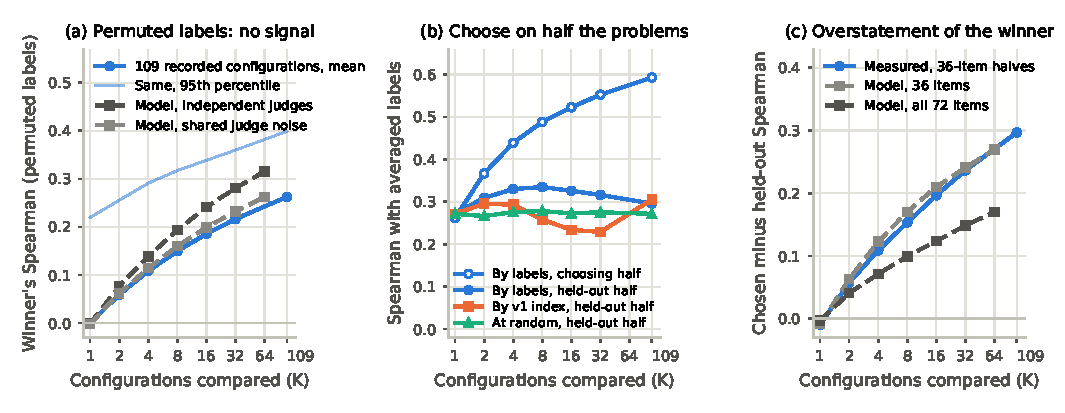
\includegraphics[width=\linewidth]{figures/best_of_k_selection_bias.pdf}
\caption{\textbf{Choosing among configurations on the validation ratings overstates the winner's agreement.} (a) Largest agreement among $K$ configurations with block-permuted ratings.
(b) Agreement of the configuration chosen on 12 problems, on those problems and on the other 12.
(c) Chosen-minus-held-out agreement, measured on half panels and simulated for half and full panels; means over 4{,}000 draws.}
\label{fig:selection-bias}
\end{figure}

% !TEX root = main.tex
\section{Additional Validation-Set Results}\label{app:moved-results}

\begin{table}[h]
  \centering
  \small
  \begin{tabular}{lcc}
    \toprule
    \textbf{Protocol}           & \textbf{Fit Spearman} & \textbf{Test Spearman} \\
    \midrule
    pass1 \(\rightarrow\) pass2 & 0.881                 & 0.810                  \\
    pass2 \(\rightarrow\) pass1 & 0.857                 & 0.786                  \\
    \bottomrule
  \end{tabular}
  \caption{\textbf{Cross-pass robustness of a weight-tuned geometric variant} (not \(\mathrm{TI}_{\mathrm{var}}\)).
  Weights over six property scores are tuned on one pass by random search; \emph{Fit Spearman} is the in-sample judge-level Spearman between the tuned index and human agreement on that pass, and \emph{Test Spearman} is the same statistic on the other pass.
  Both passes are one annotator's ratings of the same 72 pairs at two rubric strictness levels, so the test pass checks robustness to rubric strictness, not generalization to new items or raters.}
  \label{tab:cross_pass_generalization}
\end{table}

\begin{table}[h]
  \centering
  \small
  \begin{tabular}{lcc}
    \toprule
    \textbf{Threshold} & \textbf{Flip Rate (95\% CI)}                        & \textbf{Pass Rate (95\% CI)} \\
    \midrule
    0.60               & 0.058 \([0.048, 0.069]\)                            & 0.583 \([0.559, 0.608]\)     \\
    0.70               & 0.049 \([0.040, 0.059]\)                            & 0.559 \([0.537, 0.581]\)     \\
    0.80               & 0.051 \([0.042, 0.061]\)                            & 0.544 \([0.523, 0.566]\)     \\
    0.85               & \textbf{0.046} \([\textbf{0.037}, \textbf{0.057}]\) & 0.536 \([0.515, 0.557]\)     \\
    \bottomrule
  \end{tabular}
  \caption{\textbf{Threshold selection.} Stricter thresholds slightly reduce decision flips across repeated calls at a moderate cost in pass rate; bug-ladder ranking is unchanged (\(\rho_{\text{bug}}=-0.790\) at every threshold).}
  \label{tab:exp13_threshold_sweep}
\end{table}


% !TEX root = main.tex
\section{Human Agreement and Additional Judge Panels}\label{app:exp16-exp17}
\subsection{Agreement between annotation passes}\label{app:human-agreement}
Table~\ref{tab:app-human-human-ceiling} reports the frozen agreement statistics on 72 shared analyzed pairs.
The passes reflect different rubric strictness levels from the same annotator, rather than independent draws from a rater population.
Their disagreement cannot identify a numerical ceiling on model agreement.
The original rubric text remains unavailable.

\begin{table}[H]
\centering\small
\begin{tabular}{@{}lrc@{}}
\toprule
Statistic & Estimate & 95\% bootstrap interval \\
\midrule
Spearman correlation & 0.249 & $[-0.015,0.489]$ \\
Pearson correlation & 0.375 & $[0.076,0.604]$ \\
Kendall correlation & 0.221 & $[-0.016,0.442]$ \\
Quadratic-weighted $\kappa$ & 0.372 & $[0.073,0.581]$ \\
Mean absolute error & 0.771 & Not reported \\
\bottomrule
\end{tabular}
\caption{The two human passes disagree on the same artifacts, making the choice of label view consequential.
Mean absolute error uses the original $0$--$5$ rating scale; all estimates use 72 overlapping pairs.}
\label{tab:app-human-human-ceiling}
\end{table}

\subsection{Expanded configuration panel}\label{app:expanded-panel}
The expanded panel compares the arithmetic $v2$ with the pass1-selected geometric form $\mathrm{mono}^{0.4}\mathrm{stab}^{0.6}$.
Its averaged-label association is $0.769$, with bootstrap interval $[0.34,0.95]$ (Figure~\ref{fig:app-exp25-13judge}).
The result concerns 13 configurations on reused validation labels, not 13 independent model families or unseen data.
The plotted geometric index is not $\mathrm{TI}_{\mathrm{var}}$.

\begin{figure}[htbp]
\centering
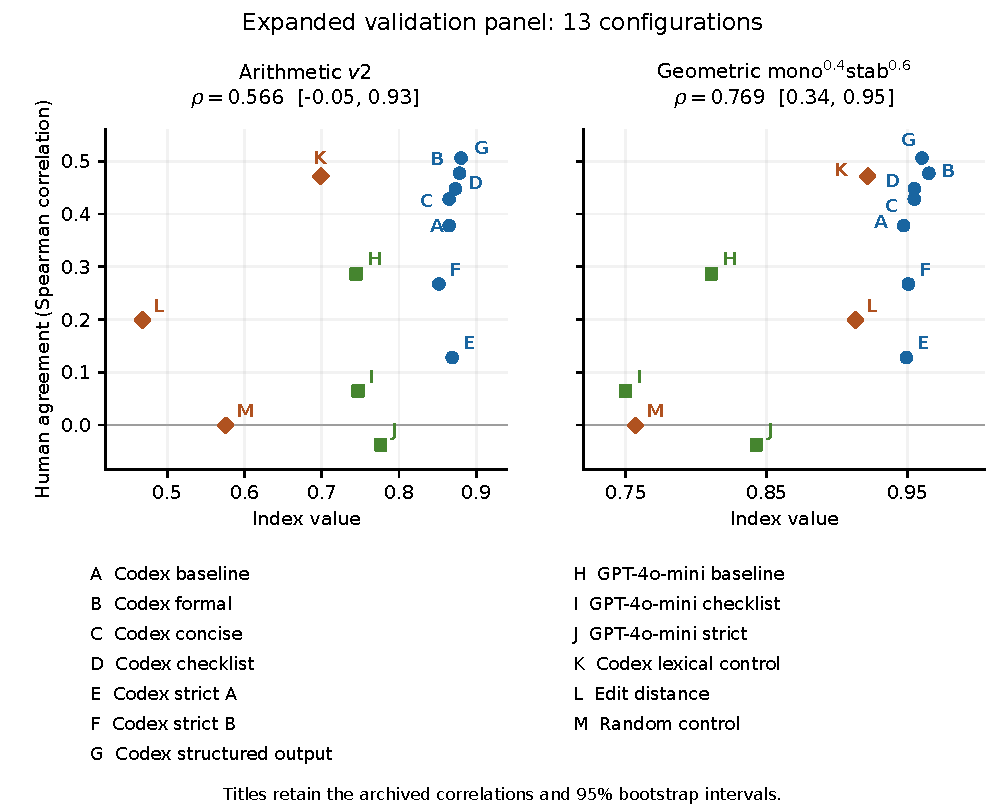
\includegraphics[width=\linewidth]{figures/expanded_panel_v2_vs_geometric.pdf}
\caption{The tuned geometric comparison has a positive association on the expanded validation panel.
The two panels compare arithmetic $v2$ with $\mathrm{mono}^{0.4}\mathrm{stab}^{0.6}$ across 13 configurations; the figure retains the archived estimates and intervals.}
\label{fig:app-exp25-13judge}
\end{figure}

\subsection{Negative results}\label{app:negative-results}
A separate Leanstral panel yields $\mathrm{TI}_{\mathrm{var}}$ associations of $-0.1190$, $-0.0476$, and $-0.0952$ on pass1, pass2, and averaged labels.
It uses \texttt{labs-leanstral-2603} in the same eight-configuration form, with three recorded scores per row for every configuration and median aggregation.
Its five-configuration semantic subset remains negatively associated on all three label views (Table~\ref{tab:subset-diagnostics}).
These recorded results contradict a claim that the fixed index works for every family.
They do not establish why the association fails.
The different-rubric human pool described in Section~\ref{sec:limitations-test} also produced no qualifying index in either registered screen.
The 32-configuration screen's largest absolute association is negative, so its sign does not support the proposed direction of the screen even before accounting for multiple comparisons.

\subsection{Can model raters substitute for human raters?}\label{app:model-raters-substitution}
Human ratings are the binding cost in judge validation, so a natural scaling route is to let frontier models stand in for the human raters and validate the judge against them.
We report a direct test of that route, run on VeriBench VBV1 (experiment 106), because the result bears on any attempt to scale judge validation without additional human ratings.
The motivating obstacle is that the available human ratings cover a single agent, so they cannot answer whether a judge generalizes to agents it has not seen.

\paragraph{Design.}
Seven frontier models, one per model family, each rate the same artifacts under the human rating instructions, both as personas constructed from the expert raters' own scores and from the instructions alone.
Their aggregate is the stand-in panel.
A judge is then validated leave-one-agent-out across fourteen agent groups of fifty tasks each: one group is held out, and agreement with the panel is measured on it.
Three judge arms are compared: the frozen deployed judge, a bare-instruction judge, and a judge rebuilt from scratch on every fold.
Against the panel the frozen judge reaches pooled Spearman $0.917$ $[0.888, 0.937]$ with $\mathrm{ICC}(A,1)$ $0.922$, which taken alone would read as strong evidence of generalization.

\paragraph{The anchor.}
One held-out group consists of exactly the items the expert raters scored, so on that group every judge can be measured against the stand-in panel and against the human raters on identical items.
Table~\ref{tab:app-standin-vs-human} reports both.

\begin{table}[H]
\centering\small
\begin{tabular}{@{}lcc@{}}
\toprule
Judge & vs.\ stand-in panel & vs.\ human raters \\
\midrule
Frozen deployed judge & $0.82$ & $0.772$ $[0.570, 0.901]$ \\
Rebuilt per fold & $0.91$ & $0.621$ $[0.278, 0.832]$ \\
Bare instructions & $0.86$ & $0.563$ $[0.176, 0.806]$ \\
\bottomrule
\end{tabular}
\caption{Spearman agreement of three judges on one held-out group of $75$ items, measured against the model stand-in panel and against the human raters who scored those same items.}
\label{tab:app-standin-vs-human}
\end{table}

\paragraph{Why substitution fails here.}
The panel agrees with the human raters at Spearman $0.770$ $[0.527, 0.898]$, and the judge it is grading agrees with those same raters at $0.772$ $[0.570, 0.901]$.
The substitute is therefore no more accurate than the instrument it is being used to assess, and agreement measured against it cannot separate judge quality from error the two share.
The inflation is largest for the judge that was itself built against the panel, whose agreement falls from $0.91$ to $0.621$, roughly twice the drop of the judge that was not.
Fitting a judge to model raters fits their idiosyncrasies.
Raising panel quality did not remove the problem.
Constructing the stand-in raters from the expert raters' own scores added nothing measurable over the rating instructions alone at the single-model stage, a paired difference of $-0.001$ $[-0.118, 0.109]$.
Widening the panel from one model to seven families raised its agreement with the human raters from $0.626$ to $0.770$, which only drew level with the judge.

\paragraph{What the substitute still supports.}
The failure is in the absolute level rather than in every comparison.
Pooled across the thirteen held-out agents the panel orders the three judge arms as $0.917$, $0.915$, and $0.876$ for the frozen, bare-instruction, and rebuilt arms, which selects the frozen judge and rejects the rebuilt one; the human evidence on the anchor group supports the same choice.
Differential quantities in which both arms carry the same shared error also survive: no judge or rater in this design favored its own model family by $0.05$ or more after Holm correction, with largest absolute effect $0.043$.
We therefore read model stand-ins as admissible for relative comparisons between judges and for same-family screens, and inadmissible as the reference for any reported judge--human agreement number.

\paragraph{Limits of this test.}
Human ratings exist for one agent group of $75$ items, so the per-judge ordering against human raters rests on point estimates whose intervals overlap.
A pre-registered non-inferiority comparison between the fold-built judge and an earlier out-of-fold judge was inconclusive, with difference $0.018$ $[-0.295, 0.338]$, rather than a refutation.
The direction is consistent across both the persona and instruction-only panels, but the single anchor group is itself the reason additional human ratings remain the binding requirement.

% !TEX root = main.tex
\section{Judge Certification: Additional Plots}\label{app:judge-cert}
We report raw scatterplots used during certification of the LLM judge.
These plots visualize the judge’s response to controlled perturbations: (P1) identity/reflexivity, (P2) cumulative bug injection, and (P3) removal of theorem statements and unit tests.
Figures A.1–A.3 show that scores drop as artifacts worsen; the bug plot is noisier with an early prompt, which motivated the simplified rubric used in the main experiments.
P4 (prompt stability/invariance) is reported in the main text with dedicated aggregate plots.

\textit{Protocol variants.} The scatterplots below are “sanity-check” runs with the simplest prompts to stress visible monotonic behavior.
In the bug study (Fig.~\ref{fig:app-bugs}) the earlier, theorem-equivalence prompt produced a noisier trend; this prompted a simplified, rubric-first prompt that we use for all reported results in the main paper, yielding the stronger correlations cited in Fig.~\ref{fig:judge_sanity_checks}.
For missing-specs (Fig.~\ref{fig:app-missing-specs}), both Claude 3.5 and 3.7 show clear negative trends; minor non-monotonicity in 3.7 disappears with the finalized rubric.

We note that, for the experiment shown in Figure \ref{fig:app-missing-specs}, a more complex judge (Claude 3.7) does not satisfy the property that the LLM Judge Score should monotonically decrease with the number of missing specs.
Indeed, the Judge File Equivalence score was not monotonic, even for Claude 3.5, leading us to simplify the rubric used in our main paper.

\begin{figure}[t]
  \centering
  \begin{subfigure}[t]{0.48\textwidth}
    \centering
    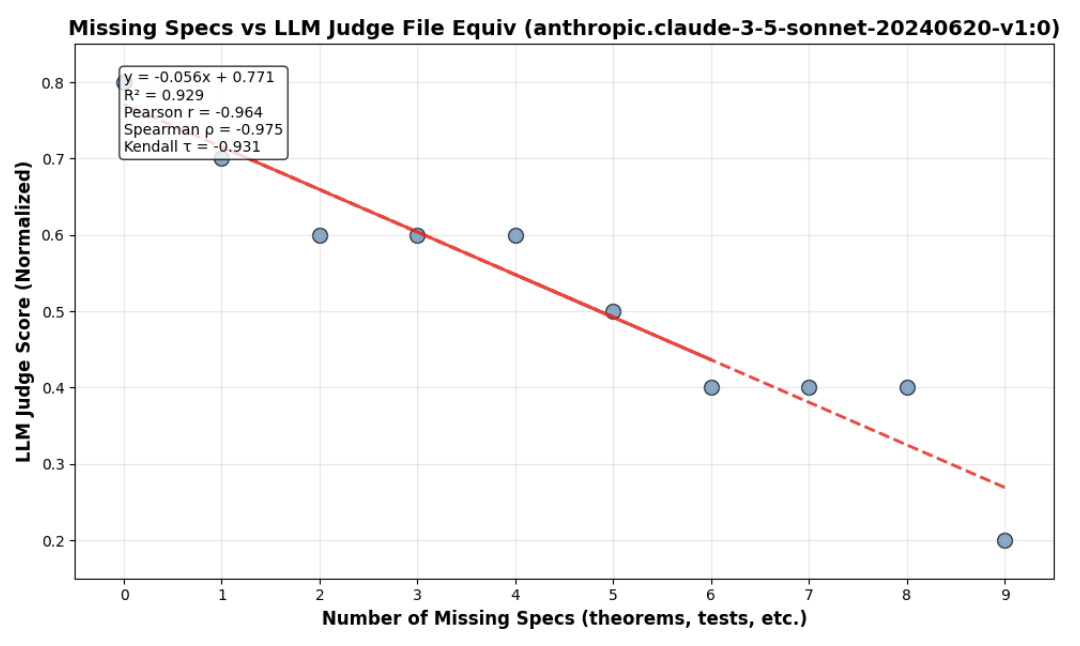
\includegraphics[width=\linewidth]{figures/3.5_specs_missing.png}
    \caption{Claude 3.5 Sonnet v1: strong monotonic decrease (\(y=-0.056x+0.771\), \(R^2=0.929\), Pearson \(r=-0.964\), Spearman \(\rho=-0.975\)).}
  \end{subfigure}\hfill
  \begin{subfigure}[t]{0.48\textwidth}
    \centering
    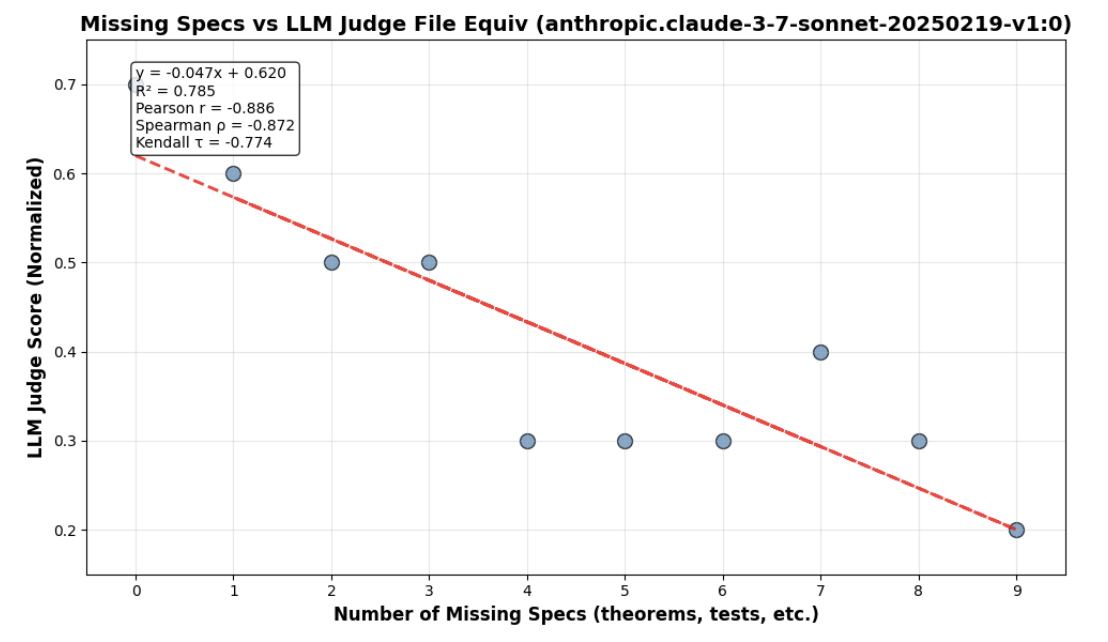
\includegraphics[width=\linewidth]{figures/3.7_specs_missing.png}
    \caption{Claude 3.7 Sonnet v1: clear negative trend with minor non-monotonicity (\(y=-0.047x+0.620\), \(R^2=0.785\), Pearson \(r=-0.886\), Spearman \(\rho=-0.872\)).}
  \end{subfigure}
  \caption{\textbf{(P3) Monotonicity w.r.t.\ missing specifications.} Candidate scores decrease as more theorems/tests are withheld.
  We retain both model variants to show robustness of the trend; 3.7’s small non-monotonicity motivated the simplified rubric used in the main results.}
  \label{fig:app-missing-specs}
\end{figure}

\begin{figure}[t]
  \centering
  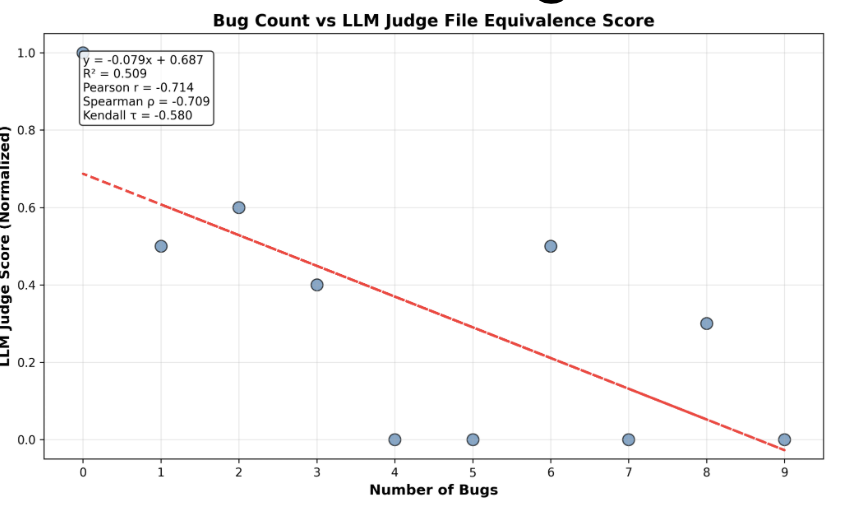
\includegraphics[width=0.85\linewidth]{figures/3.5_bugs.png}
  \caption{\textbf{(P2) Non-Monotonicity w.r.t.\ cumulative bugs (Claude 3.5 Sonnet).} Scores drop as more semantic bugs are injected (Pearson \(r=-0.714\), Spearman \(\rho=-0.709\), \(R^2=0.509\)); the higher noise with the initial “theorem-equivalence” prompt led us to simplify the rubric used for the final judge in the main paper.}
  \label{fig:app-bugs}
\end{figure}

\begin{figure}[t]
  \centering
  \begin{subfigure}[t]{0.49\textwidth}
    \centering
    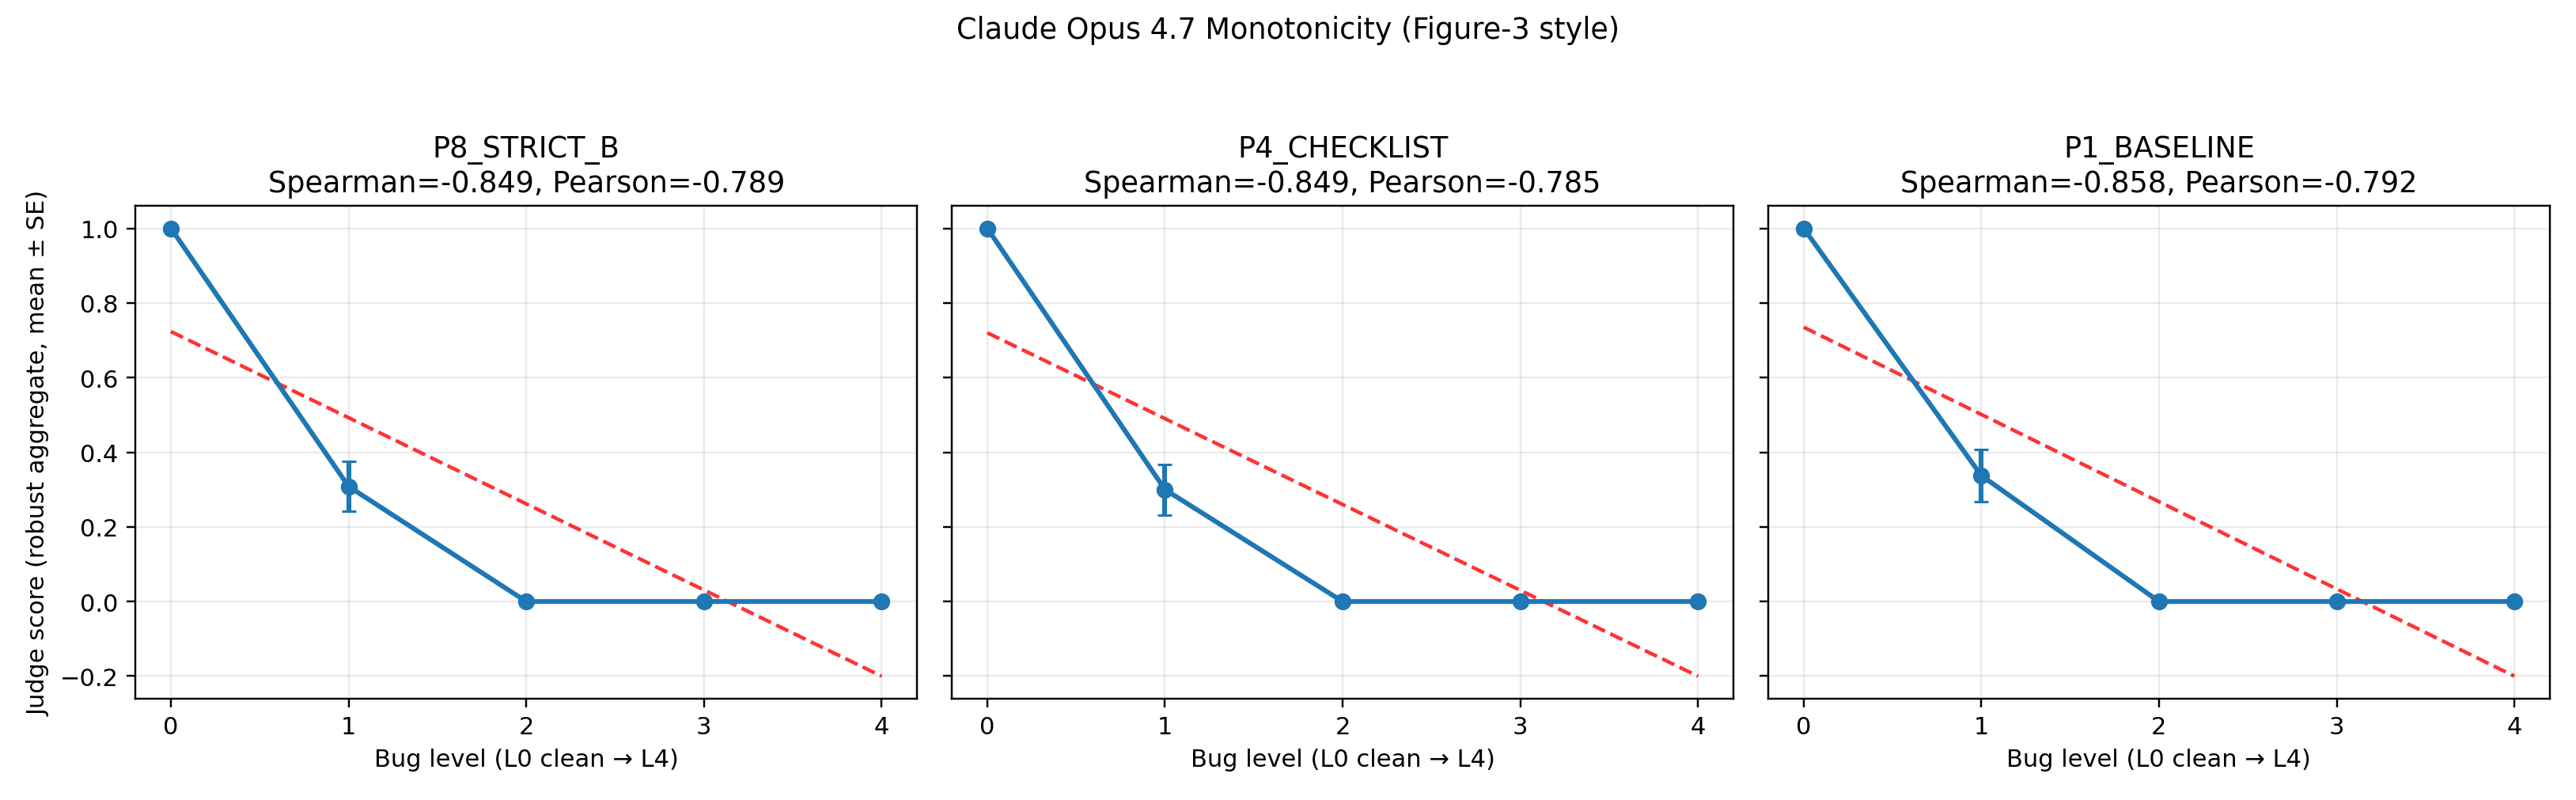
\includegraphics[width=\linewidth]{figures/fig3_style_claude_opus_monotonicity.png}
    \caption{Claude Opus 4.7 Figure-3-style monotonicity (mean \(\pm\) SE).}
  \end{subfigure}\hfill
  \begin{subfigure}[t]{0.49\textwidth}
    \centering
    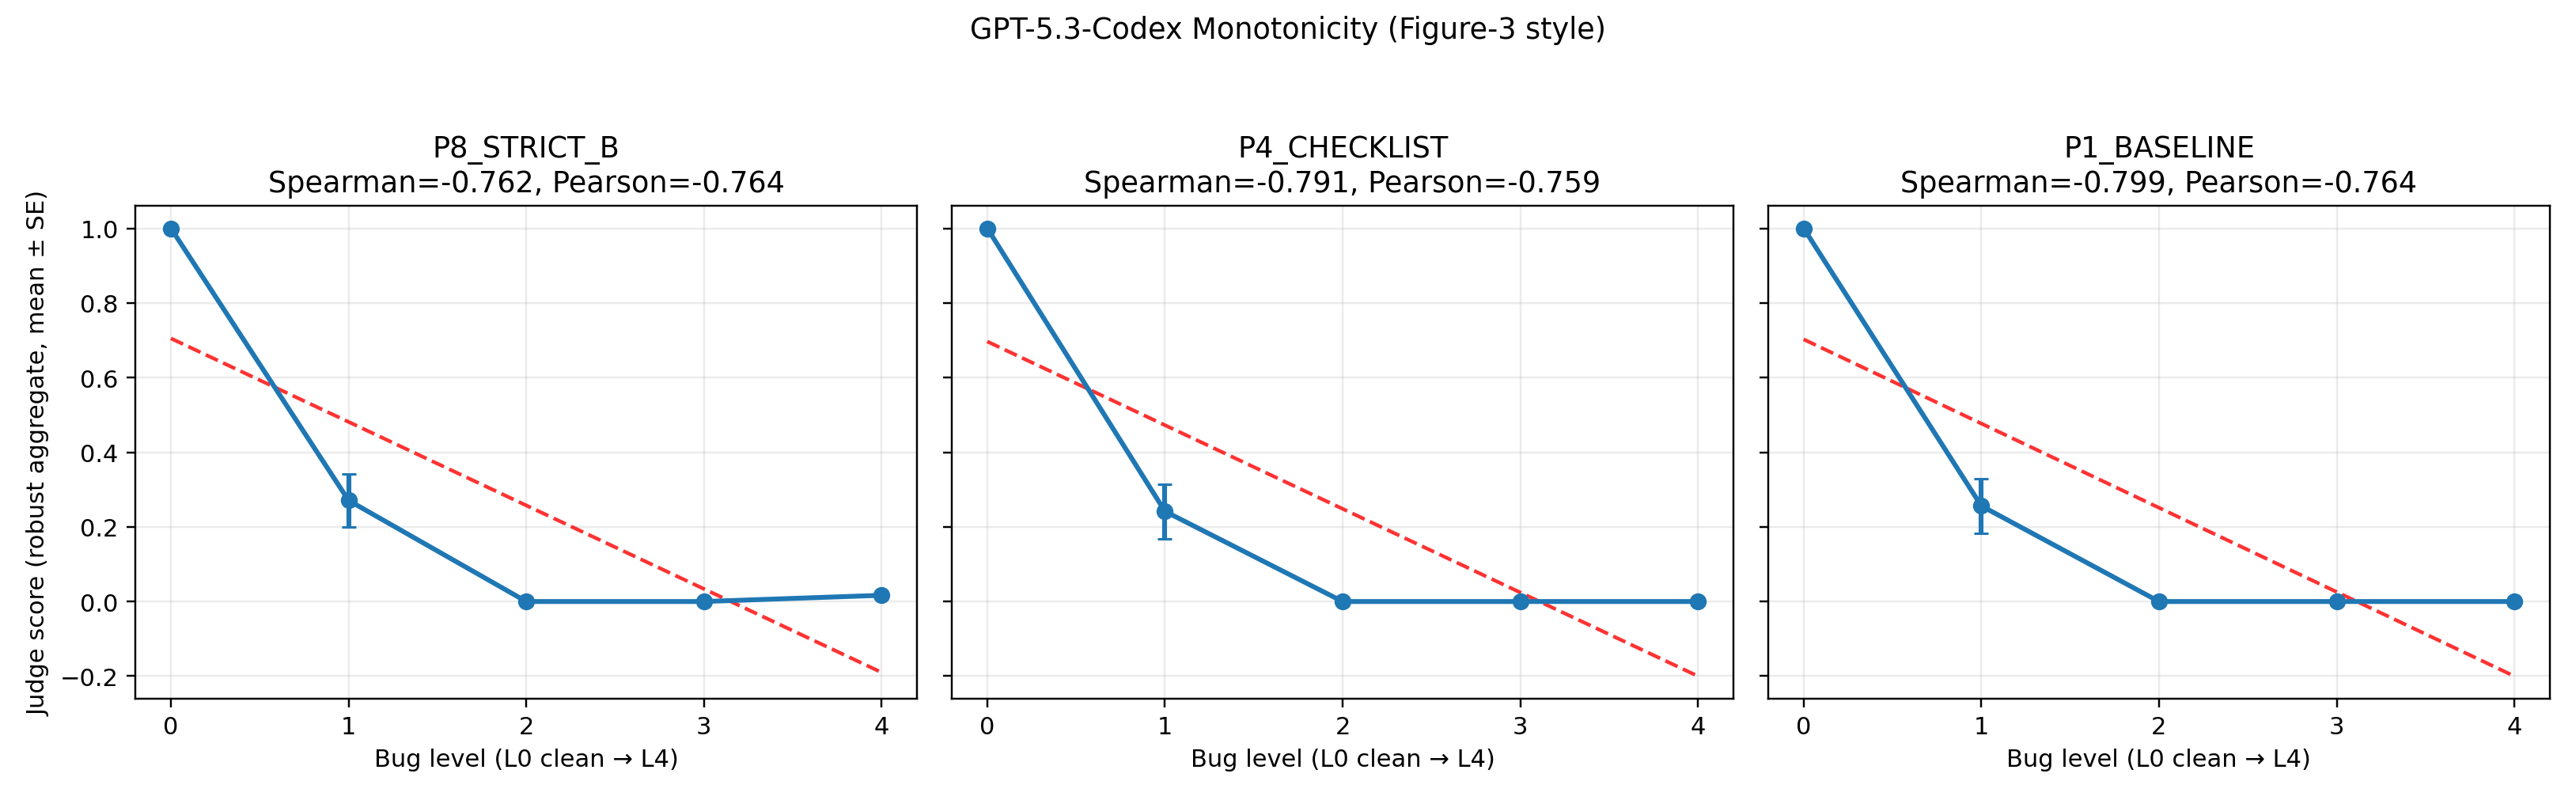
\includegraphics[width=\linewidth]{figures/fig3_style_gpt53_codex_monotonicity.png}
    \caption{GPT-5.3-Codex Figure-3-style monotonicity (mean \(\pm\) SE).}
  \end{subfigure}
  \caption{\textbf{Model-matched Figure-3-style monotonicity diagnostics.} Both judge families show strong monotone score degradation as bug intensity increases, under the same low-variance plotting protocol.}
  \label{fig:fig3_style_opus_codex}
\end{figure}

\begin{figure}[t]
  \centering
  \begin{subfigure}[t]{0.49\textwidth}
    \centering
    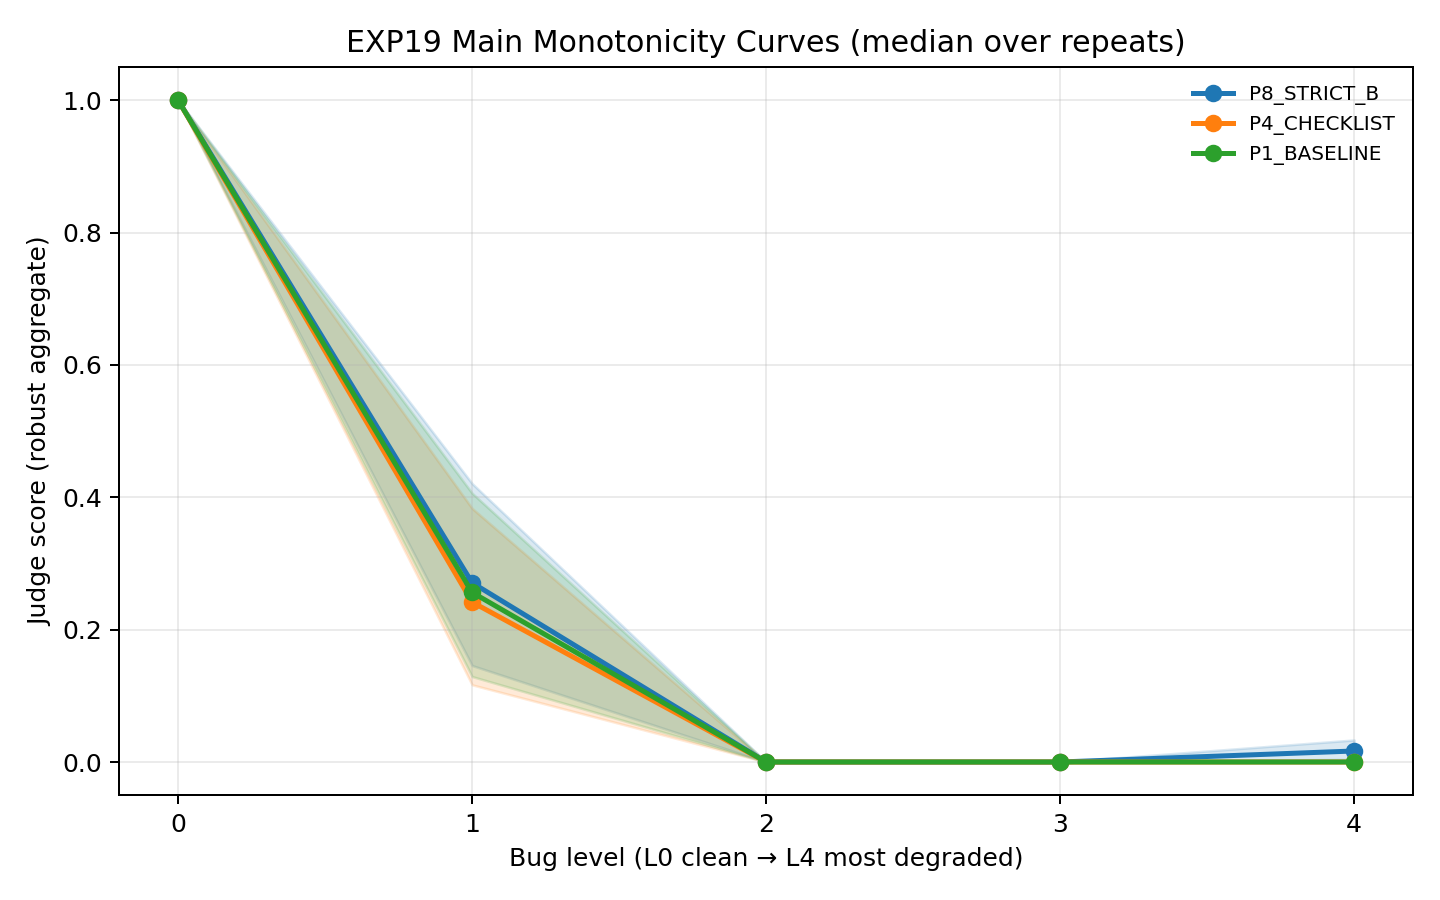
\includegraphics[width=\linewidth]{figures/fig_main_monotonicity_lowvar_codex.png}
    \caption{Codex low-variance monotonicity curves.}
  \end{subfigure}\hfill
  \begin{subfigure}[t]{0.49\textwidth}
    \centering
    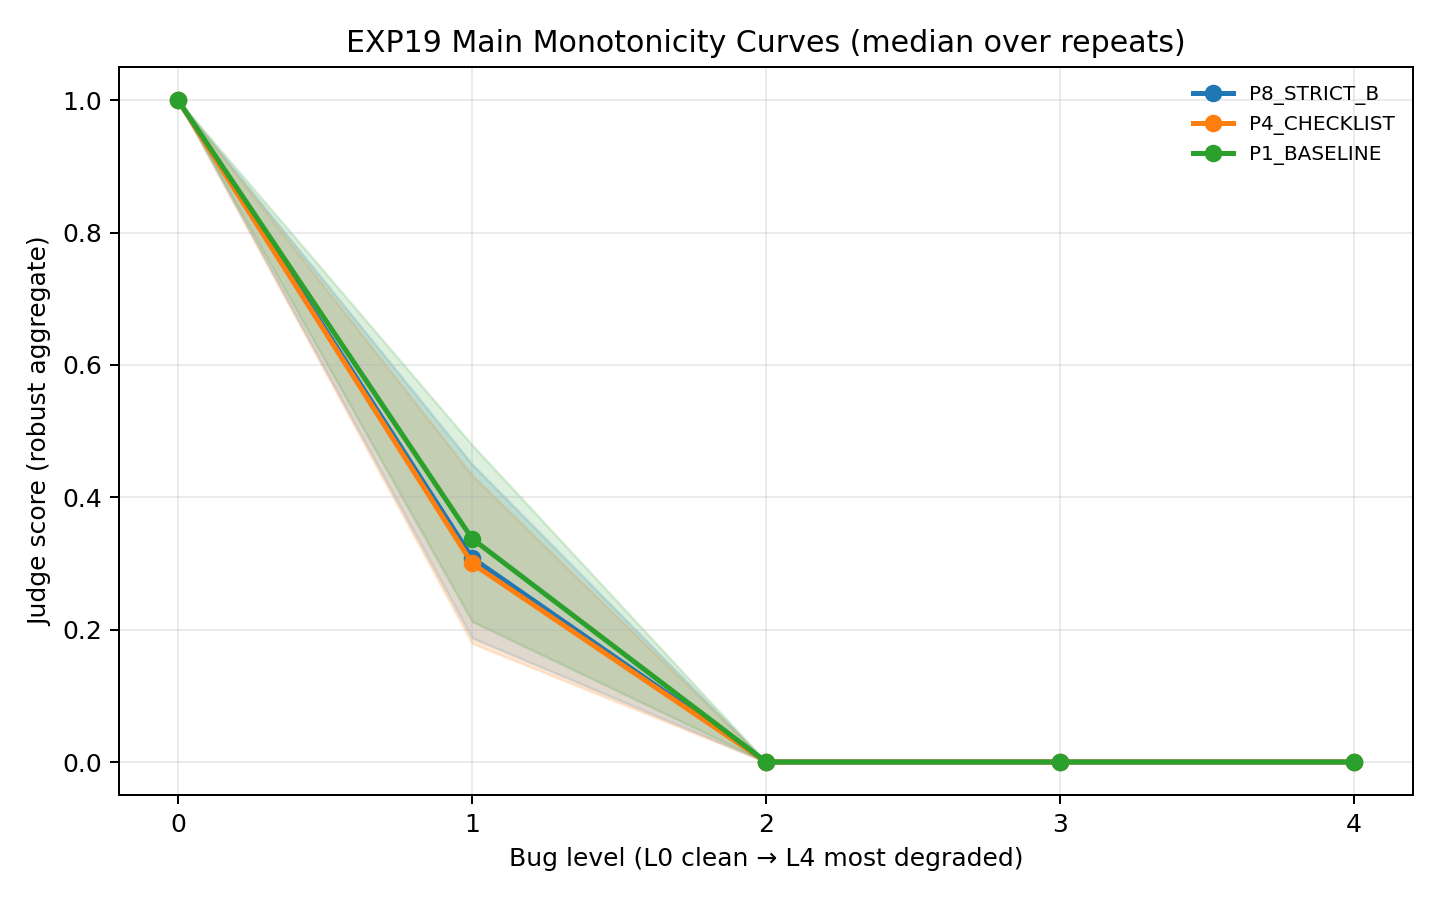
\includegraphics[width=\linewidth]{figures/fig_main_monotonicity_lowvar_opus47.png}
    \caption{Opus 4.7 low-variance monotonicity curves.}
  \end{subfigure}
  \caption{\textbf{Low-variance monotonicity trends across model families.} Both judge families show strong non-increasing behavior as bug intensity increases, under robust repeat aggregation.}
  \label{fig:lowvar_mono_codex_opus}
\end{figure}


% !TEX root = main.tex
\section{Unit Tests as Ground Theorems: A Definition We Do Not Adopt}\label{app:spec-vs-tests}
Section~\ref{sec:problem-setup} follows common formal-methods usage: the formal specification consists of theorem statements about the implementation, and unit tests are not part of it.
We record a competing view that we do not adopt.
In Lean~4, a unit test is often itself a closed theorem.
The gold \texttt{myAdd} artifact states its tests as, e.g., \texttt{example : myAdd 1 2 = 3 := by native\_decide}, an anonymous theorem with no free variables.
On this view, a unit test specifies the implementation at one concrete input, and specifications range from such ground instances to universally quantified properties such as \(\forall n,\ \texttt{myAdd}\ n\ 0 = n\).
The choice changes terminology, not our measurements.
The P3 ladder removes theorem statements and unit tests alike; under the adopted definition, only the removed theorems count as missing specification.


\end{document}
